\PassOptionsToPackage{unicode=true}{hyperref} % options for packages loaded elsewhere
\PassOptionsToPackage{hyphens}{url}
%
\documentclass[]{article}
\usepackage{lmodern}
\usepackage{amssymb,amsmath}
\usepackage{ifxetex,ifluatex}
\usepackage{fixltx2e} % provides \textsubscript
\ifnum 0\ifxetex 1\fi\ifluatex 1\fi=0 % if pdftex
  \usepackage[T1]{fontenc}
  \usepackage[utf8]{inputenc}
  \usepackage{textcomp} % provides euro and other symbols
\else % if luatex or xelatex
  \usepackage{unicode-math}
  \defaultfontfeatures{Ligatures=TeX,Scale=MatchLowercase}
\fi
% use upquote if available, for straight quotes in verbatim environments
\IfFileExists{upquote.sty}{\usepackage{upquote}}{}
% use microtype if available
\IfFileExists{microtype.sty}{%
\usepackage[]{microtype}
\UseMicrotypeSet[protrusion]{basicmath} % disable protrusion for tt fonts
}{}
\IfFileExists{parskip.sty}{%
\usepackage{parskip}
}{% else
\setlength{\parindent}{0pt}
\setlength{\parskip}{6pt plus 2pt minus 1pt}
}
\usepackage{hyperref}
\hypersetup{
            pdftitle={Constructing a DAG for Anoxic Duration Under Ice and the Concentration of Dissolved Organic Matter in Fall},
            pdfauthor={Katie Gannon},
            pdfborder={0 0 0},
            breaklinks=true}
\urlstyle{same}  % don't use monospace font for urls
\usepackage[margin=1in]{geometry}
\usepackage{color}
\usepackage{fancyvrb}
\newcommand{\VerbBar}{|}
\newcommand{\VERB}{\Verb[commandchars=\\\{\}]}
\DefineVerbatimEnvironment{Highlighting}{Verbatim}{commandchars=\\\{\}}
% Add ',fontsize=\small' for more characters per line
\usepackage{framed}
\definecolor{shadecolor}{RGB}{248,248,248}
\newenvironment{Shaded}{\begin{snugshade}}{\end{snugshade}}
\newcommand{\AlertTok}[1]{\textcolor[rgb]{0.94,0.16,0.16}{#1}}
\newcommand{\AnnotationTok}[1]{\textcolor[rgb]{0.56,0.35,0.01}{\textbf{\textit{#1}}}}
\newcommand{\AttributeTok}[1]{\textcolor[rgb]{0.77,0.63,0.00}{#1}}
\newcommand{\BaseNTok}[1]{\textcolor[rgb]{0.00,0.00,0.81}{#1}}
\newcommand{\BuiltInTok}[1]{#1}
\newcommand{\CharTok}[1]{\textcolor[rgb]{0.31,0.60,0.02}{#1}}
\newcommand{\CommentTok}[1]{\textcolor[rgb]{0.56,0.35,0.01}{\textit{#1}}}
\newcommand{\CommentVarTok}[1]{\textcolor[rgb]{0.56,0.35,0.01}{\textbf{\textit{#1}}}}
\newcommand{\ConstantTok}[1]{\textcolor[rgb]{0.00,0.00,0.00}{#1}}
\newcommand{\ControlFlowTok}[1]{\textcolor[rgb]{0.13,0.29,0.53}{\textbf{#1}}}
\newcommand{\DataTypeTok}[1]{\textcolor[rgb]{0.13,0.29,0.53}{#1}}
\newcommand{\DecValTok}[1]{\textcolor[rgb]{0.00,0.00,0.81}{#1}}
\newcommand{\DocumentationTok}[1]{\textcolor[rgb]{0.56,0.35,0.01}{\textbf{\textit{#1}}}}
\newcommand{\ErrorTok}[1]{\textcolor[rgb]{0.64,0.00,0.00}{\textbf{#1}}}
\newcommand{\ExtensionTok}[1]{#1}
\newcommand{\FloatTok}[1]{\textcolor[rgb]{0.00,0.00,0.81}{#1}}
\newcommand{\FunctionTok}[1]{\textcolor[rgb]{0.00,0.00,0.00}{#1}}
\newcommand{\ImportTok}[1]{#1}
\newcommand{\InformationTok}[1]{\textcolor[rgb]{0.56,0.35,0.01}{\textbf{\textit{#1}}}}
\newcommand{\KeywordTok}[1]{\textcolor[rgb]{0.13,0.29,0.53}{\textbf{#1}}}
\newcommand{\NormalTok}[1]{#1}
\newcommand{\OperatorTok}[1]{\textcolor[rgb]{0.81,0.36,0.00}{\textbf{#1}}}
\newcommand{\OtherTok}[1]{\textcolor[rgb]{0.56,0.35,0.01}{#1}}
\newcommand{\PreprocessorTok}[1]{\textcolor[rgb]{0.56,0.35,0.01}{\textit{#1}}}
\newcommand{\RegionMarkerTok}[1]{#1}
\newcommand{\SpecialCharTok}[1]{\textcolor[rgb]{0.00,0.00,0.00}{#1}}
\newcommand{\SpecialStringTok}[1]{\textcolor[rgb]{0.31,0.60,0.02}{#1}}
\newcommand{\StringTok}[1]{\textcolor[rgb]{0.31,0.60,0.02}{#1}}
\newcommand{\VariableTok}[1]{\textcolor[rgb]{0.00,0.00,0.00}{#1}}
\newcommand{\VerbatimStringTok}[1]{\textcolor[rgb]{0.31,0.60,0.02}{#1}}
\newcommand{\WarningTok}[1]{\textcolor[rgb]{0.56,0.35,0.01}{\textbf{\textit{#1}}}}
\usepackage{longtable,booktabs}
% Fix footnotes in tables (requires footnote package)
\IfFileExists{footnote.sty}{\usepackage{footnote}\makesavenoteenv{longtable}}{}
\usepackage{graphicx,grffile}
\makeatletter
\def\maxwidth{\ifdim\Gin@nat@width>\linewidth\linewidth\else\Gin@nat@width\fi}
\def\maxheight{\ifdim\Gin@nat@height>\textheight\textheight\else\Gin@nat@height\fi}
\makeatother
% Scale images if necessary, so that they will not overflow the page
% margins by default, and it is still possible to overwrite the defaults
% using explicit options in \includegraphics[width, height, ...]{}
\setkeys{Gin}{width=\maxwidth,height=\maxheight,keepaspectratio}
\setlength{\emergencystretch}{3em}  % prevent overfull lines
\providecommand{\tightlist}{%
  \setlength{\itemsep}{0pt}\setlength{\parskip}{0pt}}
\setcounter{secnumdepth}{0}
% Redefines (sub)paragraphs to behave more like sections
\ifx\paragraph\undefined\else
\let\oldparagraph\paragraph
\renewcommand{\paragraph}[1]{\oldparagraph{#1}\mbox{}}
\fi
\ifx\subparagraph\undefined\else
\let\oldsubparagraph\subparagraph
\renewcommand{\subparagraph}[1]{\oldsubparagraph{#1}\mbox{}}
\fi

% set default figure placement to htbp
\makeatletter
\def\fps@figure{htbp}
\makeatother


\title{Constructing a DAG for Anoxic Duration Under Ice and the Concentration
of Dissolved Organic Matter in Fall}
\author{Katie Gannon}
\date{2025-02-05}

\begin{document}
\maketitle

\hypertarget{setting-up-r-environment}{%
\section{Setting Up R Environment}\label{setting-up-r-environment}}

\begin{Shaded}
\begin{Highlighting}[]
\KeywordTok{library}\NormalTok{(ggdag)}
\end{Highlighting}
\end{Shaded}

\begin{verbatim}
## 
## Attaching package: 'ggdag'
\end{verbatim}

\begin{verbatim}
## The following object is masked from 'package:stats':
## 
##     filter
\end{verbatim}

\begin{Shaded}
\begin{Highlighting}[]
\KeywordTok{require}\NormalTok{(knitr)}
\end{Highlighting}
\end{Shaded}

\begin{verbatim}
## Loading required package: knitr
\end{verbatim}

\begin{Shaded}
\begin{Highlighting}[]
\KeywordTok{library}\NormalTok{(dagitty)}
\KeywordTok{require}\NormalTok{(tidyr)}
\end{Highlighting}
\end{Shaded}

\begin{verbatim}
## Loading required package: tidyr
\end{verbatim}

\begin{Shaded}
\begin{Highlighting}[]
\KeywordTok{require}\NormalTok{(ddplyr)}
\end{Highlighting}
\end{Shaded}

\begin{verbatim}
## Loading required package: ddplyr
\end{verbatim}

\begin{Shaded}
\begin{Highlighting}[]
\KeywordTok{library}\NormalTok{(tidyverse)}
\end{Highlighting}
\end{Shaded}

\begin{verbatim}
## -- Attaching core tidyverse packages ------------------------ tidyverse 2.0.0 --
## v dplyr     1.1.4     v purrr     1.0.2
## v forcats   1.0.0     v readr     2.1.4
## v ggplot2   3.5.1     v stringr   1.5.1
## v lubridate 1.9.3     v tibble    3.2.1
\end{verbatim}

\begin{verbatim}
## -- Conflicts ------------------------------------------ tidyverse_conflicts() --
## x dplyr::filter() masks ggdag::filter(), stats::filter()
## x dplyr::lag()    masks stats::lag()
## i Use the conflicted package (<http://conflicted.r-lib.org/>) to force all conflicts to become errors
\end{verbatim}

\hypertarget{project-overview}{%
\section{Project Overview}\label{project-overview}}

{ \emph{Katie Comment:} I study lakes and for one of my projects I am
interested in the processes happening under lake ice in winter. I will
be using this exercise to explore how the amount of organic matter
(measured as the concentration of dissolved organic carbon or DOC) in
the water of a lake in the fall impacts the duration of anoxia (no
oxygen) in bottom waters of mountain lakes. }

{ Here are all of the variables that I initially included in my DAG
After going through this exercise I realize that I can certainly
simplify some of these! }

\begin{longtable}[]{@{}ll@{}}
\toprule
\begin{minipage}[b]{0.19\columnwidth}\raggedright
\textbf{Variable name }\strut
\end{minipage} & \begin{minipage}[b]{0.75\columnwidth}\raggedright
\textbf{Description }\strut
\end{minipage}\tabularnewline
\midrule
\endhead
\begin{minipage}[t]{0.19\columnwidth}\raggedright
\(\text{anox_duration}\)\strut
\end{minipage} & \begin{minipage}[t]{0.75\columnwidth}\raggedright
The amount of time (measured in days) that the water at the bottom of
the lake has an oxygen concentration under 0.5 mg/L\strut
\end{minipage}\tabularnewline
\begin{minipage}[t]{0.19\columnwidth}\raggedright
\(\text{O2_at_Freeze}\)\strut
\end{minipage} & \begin{minipage}[t]{0.75\columnwidth}\raggedright
The total amount of oxygen present in the lake when the lake freezes in
the fall\strut
\end{minipage}\tabularnewline
\begin{minipage}[t]{0.19\columnwidth}\raggedright
\(\text{Ice_Duration}\)\strut
\end{minipage} & \begin{minipage}[t]{0.75\columnwidth}\raggedright
Amount of time (measured in days) that ice is on the lake in the
winter\strut
\end{minipage}\tabularnewline
\begin{minipage}[t]{0.19\columnwidth}\raggedright
\(\text{Rare of O2 Drawdown}\)\strut
\end{minipage} & \begin{minipage}[t]{0.75\columnwidth}\raggedright
NThe rate of oxygen depletion under ice\strut
\end{minipage}\tabularnewline
\begin{minipage}[t]{0.19\columnwidth}\raggedright
\(\text{Lake Volume}\)\strut
\end{minipage} & \begin{minipage}[t]{0.75\columnwidth}\raggedright
Volume of water in the lake\strut
\end{minipage}\tabularnewline
\begin{minipage}[t]{0.19\columnwidth}\raggedright
\(\text{Fall Mixing Duration}\)\strut
\end{minipage} & \begin{minipage}[t]{0.75\columnwidth}\raggedright
Number of days that the lake was fully mixed in fall\strut
\end{minipage}\tabularnewline
\begin{minipage}[t]{0.19\columnwidth}\raggedright
\(\text{Freezing Degree Days }\)\strut
\end{minipage} & \begin{minipage}[t]{0.75\columnwidth}\raggedright
Number of days when the air temperature was bellow freezing\strut
\end{minipage}\tabularnewline
\begin{minipage}[t]{0.19\columnwidth}\raggedright
\(\text{Snow Accumulation}\)\strut
\end{minipage} & \begin{minipage}[t]{0.75\columnwidth}\raggedright
Snow depth on the lake\strut
\end{minipage}\tabularnewline
\begin{minipage}[t]{0.19\columnwidth}\raggedright
\(\text{Ice Thickness}\)\strut
\end{minipage} & \begin{minipage}[t]{0.75\columnwidth}\raggedright
Thickness of ice measured in cm\strut
\end{minipage}\tabularnewline
\begin{minipage}[t]{0.19\columnwidth}\raggedright
\(\text{SWE}\)\strut
\end{minipage} & \begin{minipage}[t]{0.75\columnwidth}\raggedright
Snow water equivalents\strut
\end{minipage}\tabularnewline
\begin{minipage}[t]{0.19\columnwidth}\raggedright
\(\text{Wind}\)\strut
\end{minipage} & \begin{minipage}[t]{0.75\columnwidth}\raggedright
average windspeed at on the lake since last snowfall event\strut
\end{minipage}\tabularnewline
\begin{minipage}[t]{0.19\columnwidth}\raggedright
\(\text{ER Under Ice}\)\strut
\end{minipage} & \begin{minipage}[t]{0.75\columnwidth}\raggedright
Rate of ecosystem respiration occuring under ice\strut
\end{minipage}\tabularnewline
\begin{minipage}[t]{0.19\columnwidth}\raggedright
\(\text{GPP Under Ice}\)\strut
\end{minipage} & \begin{minipage}[t]{0.75\columnwidth}\raggedright
Rate of gross primary productivity under ice\strut
\end{minipage}\tabularnewline
\begin{minipage}[t]{0.19\columnwidth}\raggedright
\(\text{Summer GPP}\)\strut
\end{minipage} & \begin{minipage}[t]{0.75\columnwidth}\raggedright
Rate of gross primary productivity the previous summer\strut
\end{minipage}\tabularnewline
\begin{minipage}[t]{0.19\columnwidth}\raggedright
\(\text{Terrestrial DOC Inputs}\)\strut
\end{minipage} & \begin{minipage}[t]{0.75\columnwidth}\raggedright
Organic matter inputs to the lake from the watershed during summer\strut
\end{minipage}\tabularnewline
\begin{minipage}[t]{0.19\columnwidth}\raggedright
\(\text{DOC at freezing}\)\strut
\end{minipage} & \begin{minipage}[t]{0.75\columnwidth}\raggedright
Amount of organic matter present in the lake when the ice freezes
measured as concentration of dissolved organic matter\strut
\end{minipage}\tabularnewline
\bottomrule
\end{longtable}

\hypertarget{first-draft-dag}{%
\section{First Draft DAG}\label{first-draft-dag}}

\begin{Shaded}
\begin{Highlighting}[]
\CommentTok{## Specify the DAG - Version 1}
\NormalTok{DAG_oxygen_under_ice_v1 <-}\StringTok{ }\KeywordTok{dagify}\NormalTok{(}
\NormalTok{  anox_duration }\OperatorTok{~}\StringTok{ }\NormalTok{O2_at_Freeze }\OperatorTok{+}\StringTok{ }\NormalTok{Ice_Duration }\OperatorTok{+}\StringTok{ }\NormalTok{Rate_O2_Drawdown,}
\NormalTok{  O2_at_Freeze }\OperatorTok{~}\StringTok{ }\NormalTok{Lake_Volume }\OperatorTok{+}\StringTok{ }\NormalTok{Fall_Mixing_Duration,}
\NormalTok{  Ice_Duration }\OperatorTok{~}\StringTok{ }\NormalTok{Freezing_Degree_Days }\OperatorTok{+}\StringTok{ }\NormalTok{Snow_Accumulation }\OperatorTok{+}\StringTok{ }\NormalTok{Ice_Thickness, }
\NormalTok{  Snow_Accumulation }\OperatorTok{~}\StringTok{ }\NormalTok{SWE }\OperatorTok{+}\StringTok{ }\NormalTok{Wind,}
\NormalTok{  Rate_O2_Drawdown }\OperatorTok{~}\StringTok{ }\NormalTok{ER_under_ice }\OperatorTok{+}\StringTok{ }\NormalTok{GPP_under_ice, }
\NormalTok{  ER_under_ice }\OperatorTok{~}\StringTok{ }\NormalTok{Freezing_Degree_Days }\OperatorTok{+}\StringTok{ }\NormalTok{DOC_at_Freeze,}
\NormalTok{  DOC_at_Freeze }\OperatorTok{~}\StringTok{ }\NormalTok{Terrestrial_DOC_Inputs }\OperatorTok{+}\StringTok{ }\NormalTok{Summer_GPP, }
\NormalTok{  GPP_under_ice }\OperatorTok{~}\StringTok{ }\NormalTok{Summer_GPP }\OperatorTok{+}\StringTok{ }\NormalTok{Light_Availability,}
\NormalTok{  Light_Availability }\OperatorTok{~}\StringTok{ }\NormalTok{Snow_Accumulation }\OperatorTok{+}\StringTok{ }\NormalTok{Ice_Thickness}
\NormalTok{)}
\KeywordTok{plot}\NormalTok{(DAG_oxygen_under_ice_v1)}
\end{Highlighting}
\end{Shaded}

\begin{verbatim}
## Plot coordinates for graph not supplied! Generating coordinates, see ?coordinates for how to set your own.
\end{verbatim}

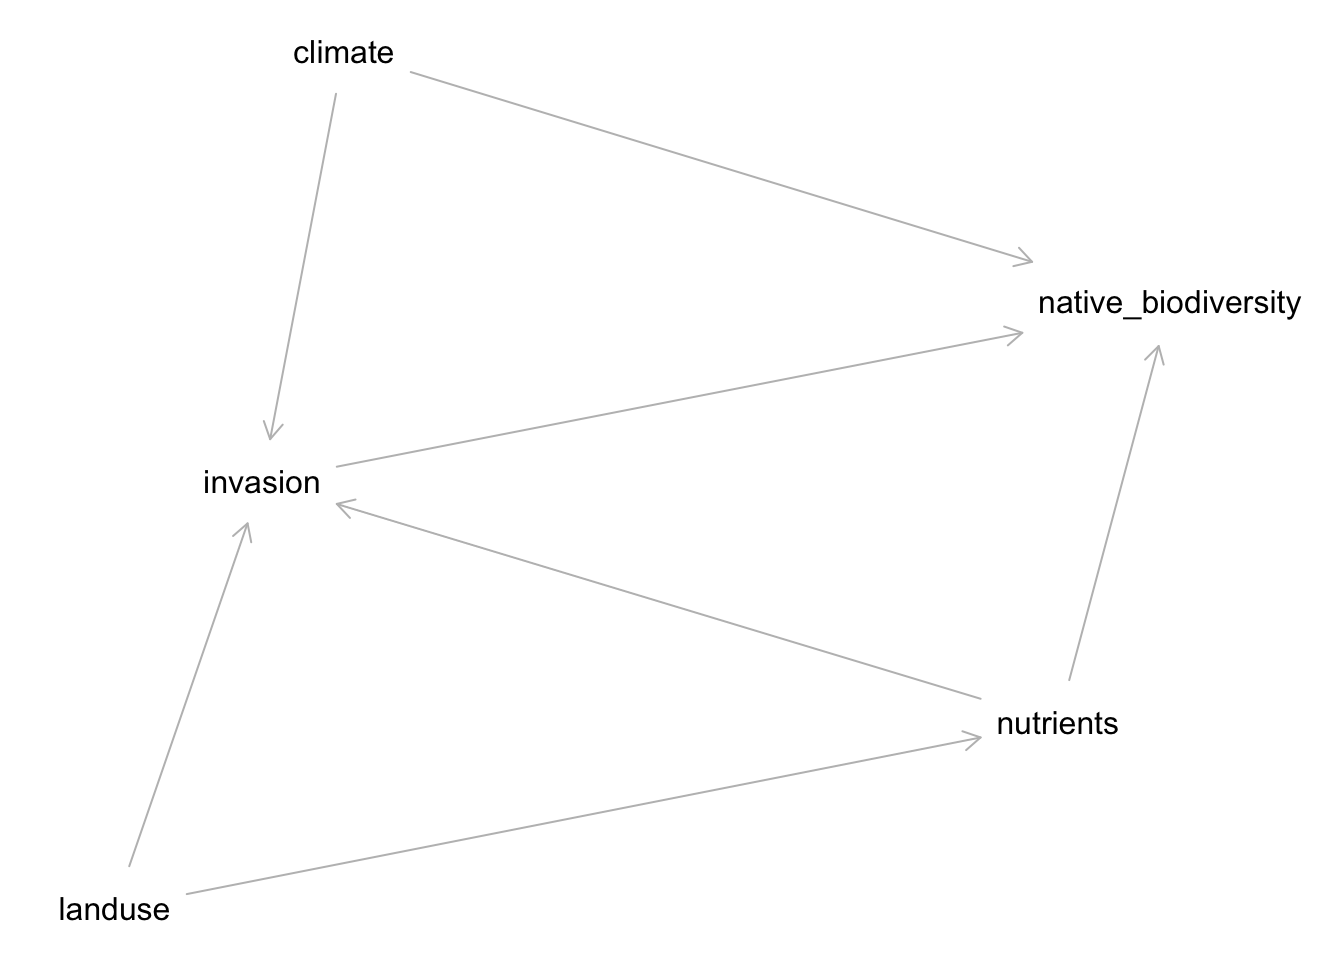
\includegraphics{01_Create_DAG_files/figure-latex/unnamed-chunk-1-1.pdf}
\# DAG Version 2

\begin{Shaded}
\begin{Highlighting}[]
\KeywordTok{set.seed}\NormalTok{(}\DecValTok{061295}\NormalTok{)}
\CommentTok{## Specify the DAG - Version 2}
\NormalTok{DAG_oxygen_under_ice_v2 <-}\StringTok{ }\KeywordTok{dagify}\NormalTok{(}
\NormalTok{  anox_duration }\OperatorTok{~}\StringTok{ }\NormalTok{O2_at_Freeze }\OperatorTok{+}\StringTok{ }\NormalTok{Ice_Duration }\OperatorTok{+}\StringTok{ }\NormalTok{Rate_O2_Drawdown,}
\NormalTok{  Rate_O2_Drawdown }\OperatorTok{~}\StringTok{ }\NormalTok{ER_under_ice }\OperatorTok{+}\StringTok{ }\NormalTok{GPP_under_ice, }
\NormalTok{  ER_under_ice }\OperatorTok{~}\StringTok{ }\NormalTok{Freezing_Degree_Days }\OperatorTok{+}\StringTok{ }\NormalTok{DOC_at_Freeze,}
\NormalTok{  DOC_at_Freeze }\OperatorTok{~}\StringTok{ }\NormalTok{Terrestrial_DOC_Inputs }\OperatorTok{+}\StringTok{ }\NormalTok{Summer_GPP, }
\NormalTok{  GPP_under_ice }\OperatorTok{~}\StringTok{ }\NormalTok{Summer_GPP }\OperatorTok{+}\StringTok{ }\NormalTok{Light_Availability,}
\NormalTok{  Light_Availability }\OperatorTok{~}\StringTok{ }\NormalTok{Snow_Accumulation }\OperatorTok{+}\StringTok{ }\NormalTok{Ice_Thickness,}
\NormalTok{  Ice_Thickness }\OperatorTok{~}\StringTok{ }\NormalTok{Freezing_Degree_Days,}
\NormalTok{  Ice_Duration }\OperatorTok{~}\StringTok{ }\NormalTok{Freezing_Degree_Days }\OperatorTok{+}\StringTok{ }\NormalTok{Snow_Accumulation, }
\NormalTok{  O2_at_Freeze }\OperatorTok{~}\StringTok{ }\NormalTok{Summer_GPP,}
\NormalTok{  Summer_GPP}\OperatorTok{~}\StringTok{ }\NormalTok{Terrestrial_DOC_Inputs}
\NormalTok{)}
\KeywordTok{plot}\NormalTok{(DAG_oxygen_under_ice_v2)}
\end{Highlighting}
\end{Shaded}

\begin{verbatim}
## Plot coordinates for graph not supplied! Generating coordinates, see ?coordinates for how to set your own.
\end{verbatim}

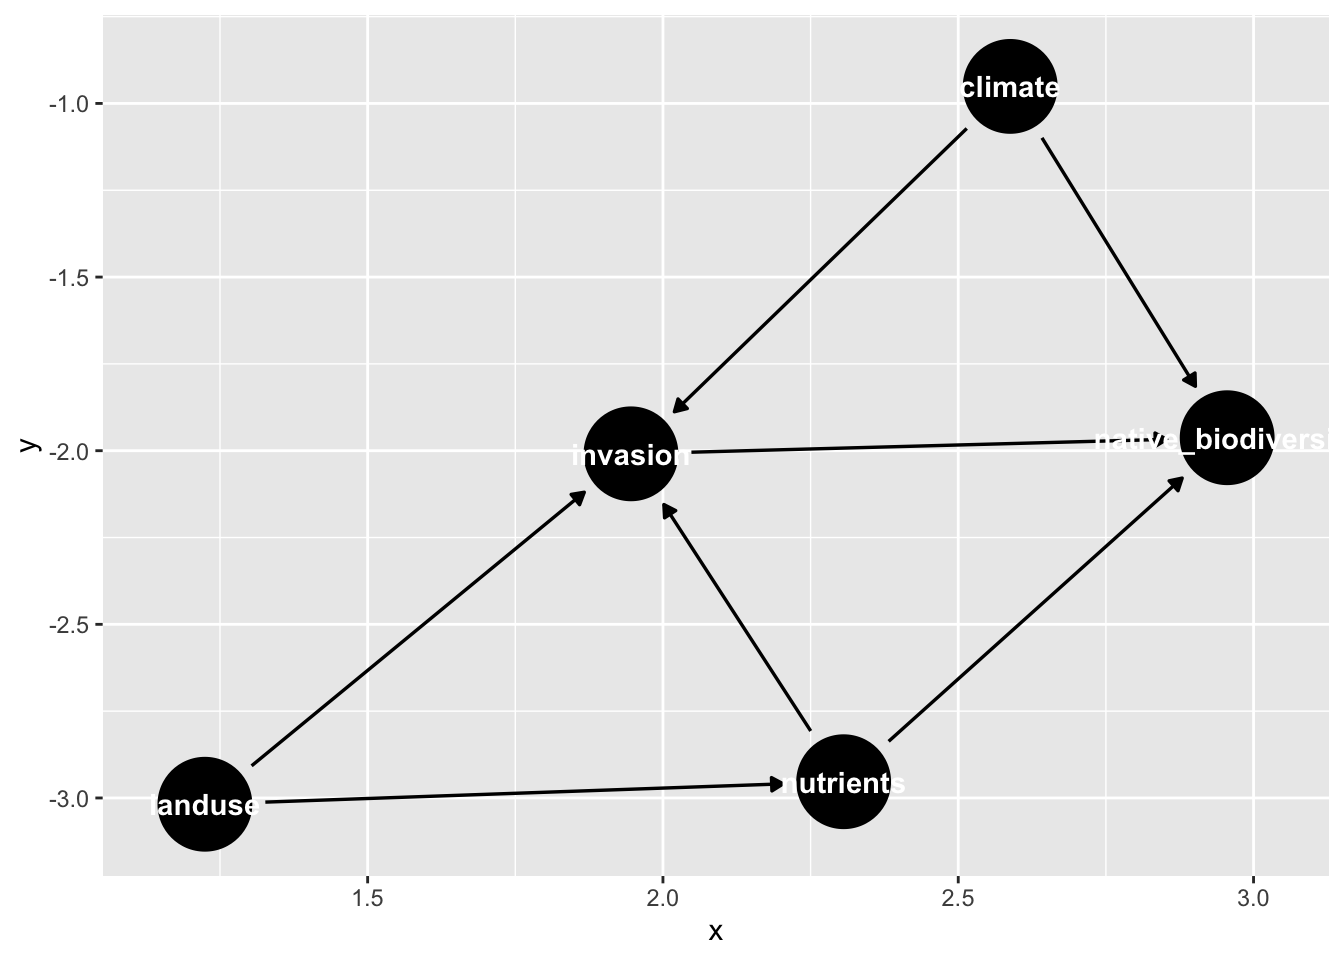
\includegraphics{01_Create_DAG_files/figure-latex/unnamed-chunk-2-1.pdf}

\hypertarget{identifying-variables-of-interest}{%
\section{Identifying Variables of
Interest}\label{identifying-variables-of-interest}}

(set the seed when plotting because otherwise the DAG shows up in
different orientations each time!)

\begin{Shaded}
\begin{Highlighting}[]
\CommentTok{# Version 1 with Labels }
\NormalTok{    DAG_oxygen_under_ice_v1 <-}\StringTok{ }\KeywordTok{dagify}\NormalTok{(}
      
      \CommentTok{#Identify Relatiobships }
\NormalTok{      anox_duration }\OperatorTok{~}\StringTok{ }\NormalTok{O2_at_Freeze }\OperatorTok{+}\StringTok{ }\NormalTok{Ice_Duration }\OperatorTok{+}\StringTok{ }\NormalTok{Rate_O2_Drawdown,}
\NormalTok{      O2_at_Freeze }\OperatorTok{~}\StringTok{ }\NormalTok{Lake_Volume }\OperatorTok{+}\StringTok{ }\NormalTok{Fall_Mixing_Duration,}
\NormalTok{      Ice_Duration }\OperatorTok{~}\StringTok{ }\NormalTok{Freezing_Degree_Days }\OperatorTok{+}\StringTok{ }\NormalTok{Snow_Accumulation }\OperatorTok{+}\StringTok{ }\NormalTok{Ice_Thickness, }
\NormalTok{      Snow_Accumulation }\OperatorTok{~}\StringTok{ }\NormalTok{SWE }\OperatorTok{+}\StringTok{ }\NormalTok{Wind,}
\NormalTok{      Rate_O2_Drawdown }\OperatorTok{~}\StringTok{ }\NormalTok{ER_under_ice }\OperatorTok{+}\StringTok{ }\NormalTok{GPP_under_ice, }
\NormalTok{      ER_under_ice }\OperatorTok{~}\StringTok{ }\NormalTok{Freezing_Degree_Days }\OperatorTok{+}\StringTok{ }\NormalTok{DOC_at_Freeze,}
\NormalTok{      DOC_at_Freeze }\OperatorTok{~}\StringTok{ }\NormalTok{Terrestrial_DOC_Inputs }\OperatorTok{+}\StringTok{ }\NormalTok{Summer_GPP, }
\NormalTok{      GPP_under_ice }\OperatorTok{~}\StringTok{ }\NormalTok{Summer_GPP }\OperatorTok{+}\StringTok{ }\NormalTok{Light_Availability,}
\NormalTok{      Light_Availability }\OperatorTok{~}\StringTok{ }\NormalTok{Snow_Accumulation }\OperatorTok{+}\StringTok{ }\NormalTok{Ice_Thickness,}
    
      \CommentTok{# Specify exposure and outcome }
      \DataTypeTok{exposure =} \StringTok{"DOC_at_Freeze"}\NormalTok{, }
      \DataTypeTok{outcome =} \StringTok{"anox_duration"}\NormalTok{,}
      
      \CommentTok{# Label }
      \DataTypeTok{labels =} \KeywordTok{c}\NormalTok{(}\DataTypeTok{outcome =} \StringTok{"Annoxic Duration"}\NormalTok{,}
                 \DataTypeTok{exposure =} \StringTok{"DOC at Lake Freeze "}\NormalTok{))}


\CommentTok{# Version 2 with labels }

\NormalTok{    DAG_oxygen_under_ice_v2 <-}\StringTok{ }\KeywordTok{dagify}\NormalTok{(}
      
      \CommentTok{#Identify Relatiobships }
\NormalTok{      anox_duration }\OperatorTok{~}\StringTok{ }\NormalTok{O2_at_Freeze }\OperatorTok{+}\StringTok{ }\NormalTok{Ice_Duration }\OperatorTok{+}\StringTok{ }\NormalTok{Rate_O2_Drawdown,}
\NormalTok{      Rate_O2_Drawdown }\OperatorTok{~}\StringTok{ }\NormalTok{ER_under_ice }\OperatorTok{+}\StringTok{ }\NormalTok{GPP_under_ice, }
\NormalTok{      ER_under_ice }\OperatorTok{~}\StringTok{ }\NormalTok{Freezing_Degree_Days }\OperatorTok{+}\StringTok{ }\NormalTok{DOC_at_Freeze,}
\NormalTok{      DOC_at_Freeze }\OperatorTok{~}\StringTok{ }\NormalTok{Terrestrial_DOC_Inputs }\OperatorTok{+}\StringTok{ }\NormalTok{Summer_GPP, }
\NormalTok{      GPP_under_ice }\OperatorTok{~}\StringTok{ }\NormalTok{Summer_GPP }\OperatorTok{+}\StringTok{ }\NormalTok{Light_Availability,}
\NormalTok{      Light_Availability }\OperatorTok{~}\StringTok{ }\NormalTok{Snow_Accumulation }\OperatorTok{+}\StringTok{ }\NormalTok{Ice_Thickness,}
\NormalTok{      Ice_Thickness }\OperatorTok{~}\StringTok{ }\NormalTok{Freezing_Degree_Days,}
\NormalTok{      Ice_Duration }\OperatorTok{~}\StringTok{ }\NormalTok{Freezing_Degree_Days }\OperatorTok{+}\StringTok{ }\NormalTok{Snow_Accumulation, }
\NormalTok{      O2_at_Freeze }\OperatorTok{~}\StringTok{ }\NormalTok{Summer_GPP,}
\NormalTok{      Summer_GPP}\OperatorTok{~}\StringTok{ }\NormalTok{Terrestrial_DOC_Inputs,}
    
      \CommentTok{# Specify exposure and outcome }
      \DataTypeTok{exposure =} \StringTok{"DOC_at_Freeze"}\NormalTok{, }
      \DataTypeTok{outcome =} \StringTok{"anox_duration"}\NormalTok{,}
      
      \CommentTok{# Label }
      \DataTypeTok{labels =} \KeywordTok{c}\NormalTok{(}\DataTypeTok{outcome =} \StringTok{"Annoxic Duration"}\NormalTok{,}
                 \DataTypeTok{exposure =} \StringTok{"DOC at Lake Freeze "}\NormalTok{))}
    
\CommentTok{# Version 3 with labels (Same DAG but slightly different question)}

\NormalTok{    DAG_oxygen_under_ice_v3 <-}\StringTok{ }\KeywordTok{dagify}\NormalTok{(}
      
      \CommentTok{#Identify Relatiobships }
\NormalTok{      anox_duration }\OperatorTok{~}\StringTok{ }\NormalTok{O2_at_Freeze }\OperatorTok{+}\StringTok{ }\NormalTok{Ice_Duration }\OperatorTok{+}\StringTok{ }\NormalTok{Rate_O2_Drawdown,}
\NormalTok{      Rate_O2_Drawdown }\OperatorTok{~}\StringTok{ }\NormalTok{ER_under_ice }\OperatorTok{+}\StringTok{ }\NormalTok{GPP_under_ice, }
\NormalTok{      ER_under_ice }\OperatorTok{~}\StringTok{ }\NormalTok{Freezing_Degree_Days }\OperatorTok{+}\StringTok{ }\NormalTok{DOC_at_Freeze,}
\NormalTok{      DOC_at_Freeze }\OperatorTok{~}\StringTok{ }\NormalTok{Terrestrial_DOC_Inputs }\OperatorTok{+}\StringTok{ }\NormalTok{Summer_GPP, }
\NormalTok{      GPP_under_ice }\OperatorTok{~}\StringTok{ }\NormalTok{Summer_GPP }\OperatorTok{+}\StringTok{ }\NormalTok{Light_Availability,}
\NormalTok{      Light_Availability }\OperatorTok{~}\StringTok{ }\NormalTok{Snow_Accumulation }\OperatorTok{+}\StringTok{ }\NormalTok{Ice_Thickness,}
\NormalTok{      Ice_Thickness }\OperatorTok{~}\StringTok{ }\NormalTok{Freezing_Degree_Days,}
\NormalTok{      Ice_Duration }\OperatorTok{~}\StringTok{ }\NormalTok{Freezing_Degree_Days }\OperatorTok{+}\StringTok{ }\NormalTok{Snow_Accumulation, }
\NormalTok{      O2_at_Freeze }\OperatorTok{~}\StringTok{ }\NormalTok{Summer_GPP,}
\NormalTok{      Summer_GPP}\OperatorTok{~}\StringTok{ }\NormalTok{Terrestrial_DOC_Inputs,}
    
      \CommentTok{# Specify exposure and outcome }
      \DataTypeTok{exposure =} \StringTok{"Summer_GPP"}\NormalTok{, }
      \DataTypeTok{outcome =} \StringTok{"anox_duration"}\NormalTok{,}
      
      \CommentTok{# Label }
      \DataTypeTok{labels =} \KeywordTok{c}\NormalTok{(}\DataTypeTok{outcome =} \StringTok{"Annoxic Duration"}\NormalTok{,}
                 \DataTypeTok{exposure =} \StringTok{"Summer GPP"}\NormalTok{))}

\CommentTok{# Visualize both versions }
\KeywordTok{set.seed}\NormalTok{(}\DecValTok{124}\NormalTok{)}

\KeywordTok{ggdag_status}\NormalTok{(DAG_oxygen_under_ice_v1,}
             \DataTypeTok{use_labels =} \StringTok{"label"}\NormalTok{,}
             \DataTypeTok{text =} \OtherTok{TRUE}\NormalTok{,}
             \DataTypeTok{text_col =} \StringTok{"black"}\NormalTok{,}
             \DataTypeTok{label_alpha =} \FloatTok{0.5}\NormalTok{) }\OperatorTok{+}\StringTok{ }\KeywordTok{theme_dag}\NormalTok{()}
\end{Highlighting}
\end{Shaded}

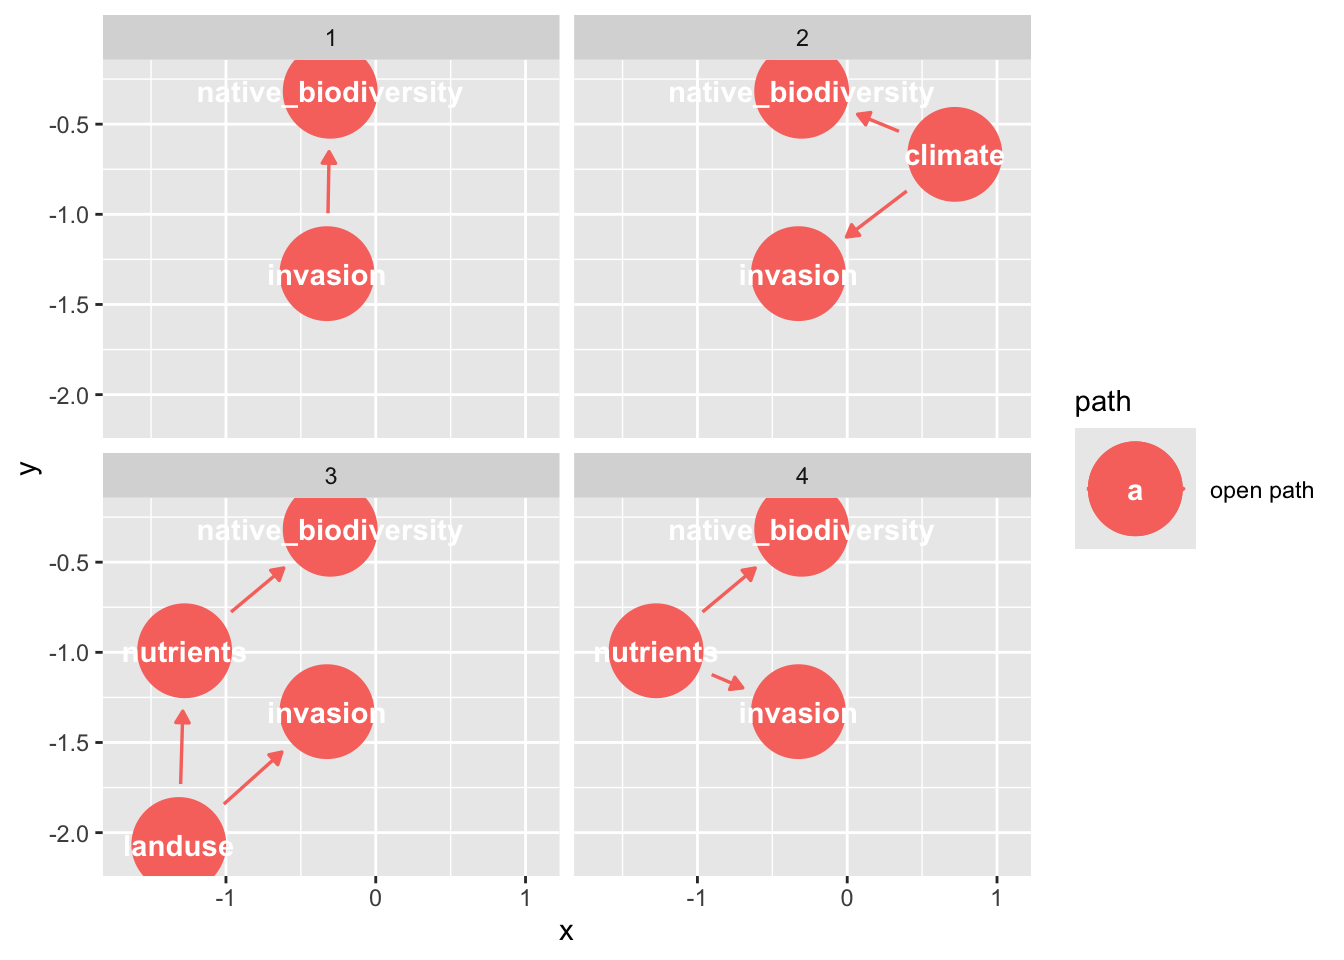
\includegraphics{01_Create_DAG_files/figure-latex/unnamed-chunk-3-1.pdf}

\begin{Shaded}
\begin{Highlighting}[]
\KeywordTok{ggdag_status}\NormalTok{(DAG_oxygen_under_ice_v2,}
             \DataTypeTok{use_labels =} \StringTok{"label"}\NormalTok{,}
             \DataTypeTok{text =} \OtherTok{TRUE}\NormalTok{,}
              \DataTypeTok{text_col =} \StringTok{"black"}\NormalTok{,}
             \DataTypeTok{label_alpha =} \FloatTok{0.5}\NormalTok{) }\OperatorTok{+}\StringTok{ }\KeywordTok{theme_dag}\NormalTok{()}
\end{Highlighting}
\end{Shaded}

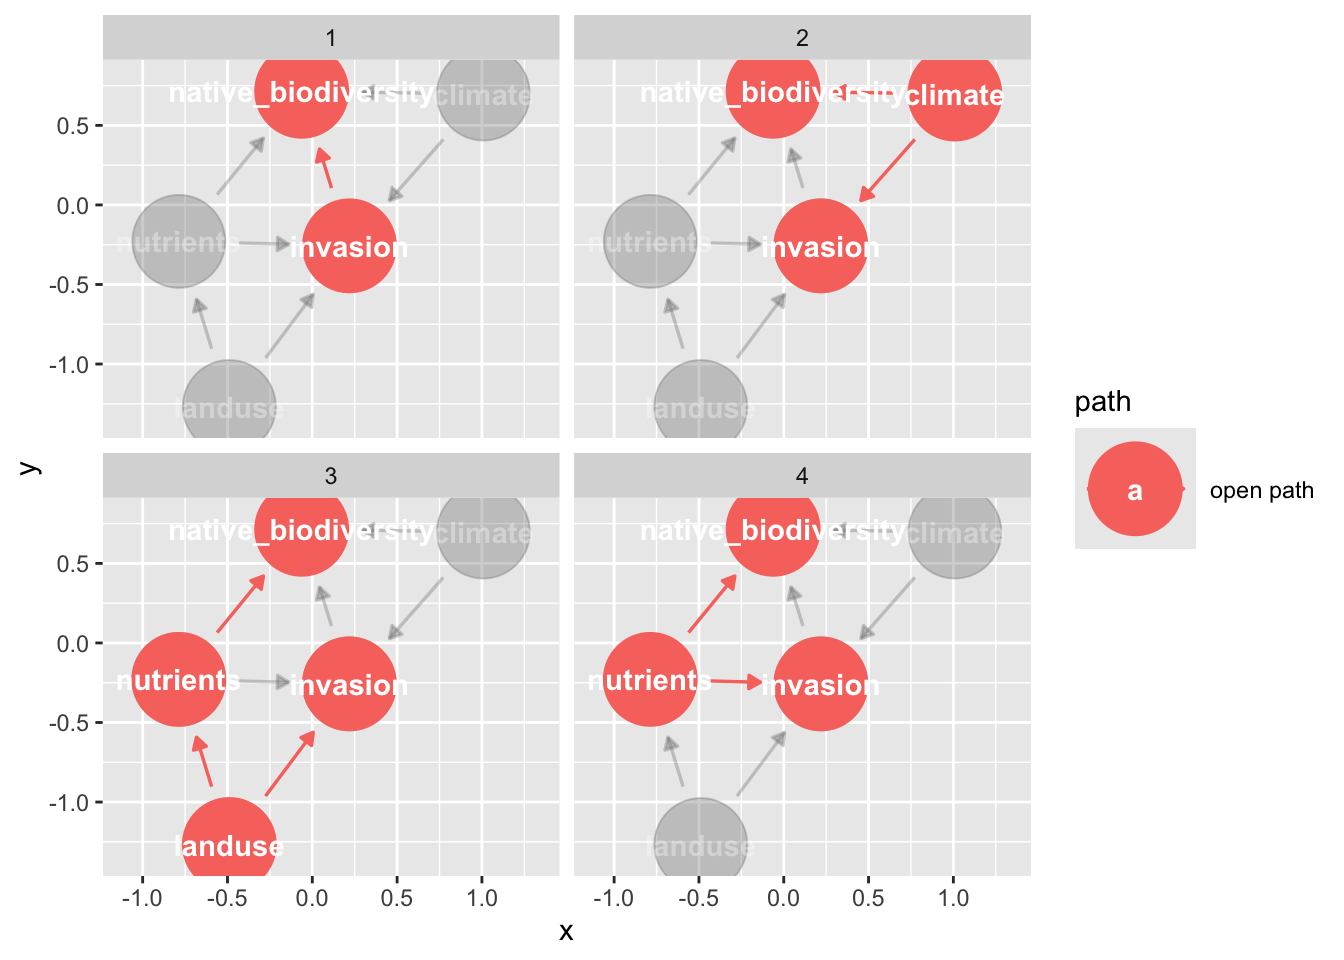
\includegraphics{01_Create_DAG_files/figure-latex/unnamed-chunk-3-2.pdf}

\begin{Shaded}
\begin{Highlighting}[]
\KeywordTok{ggdag_status}\NormalTok{(DAG_oxygen_under_ice_v3,}
             \DataTypeTok{use_labels =} \StringTok{"label"}\NormalTok{,}
             \DataTypeTok{text =} \OtherTok{TRUE}\NormalTok{,}
              \DataTypeTok{text_col =} \StringTok{"black"}\NormalTok{,}
             \DataTypeTok{label_alpha =} \FloatTok{0.5}\NormalTok{) }\OperatorTok{+}\StringTok{ }\KeywordTok{theme_dag}\NormalTok{()}
\end{Highlighting}
\end{Shaded}

\includegraphics{01_Create_DAG_files/figure-latex/unnamed-chunk-3-3.pdf}

{ \emph{Katie Comment:} Cool! I have a DAG! It is a bit of a mess at the
momment because I think there are some extra variables that I don't need
to worry about still hanging around in the DAG. As we move forward and
refine things I might be able to make this prettier!\\
}

\#Identify what must be controled for using adjustmentSets(). We can
also have a summary of all possible paths in the DAG and identify which
are open vs closed backdoors using paths(). This function takes a DAG,
with a given ``exposure'' or ``treatment variable'' and an ``outcome''
and identifies open backdoors: confounding variables (common causes)
that need to be controlled for.

\begin{Shaded}
\begin{Highlighting}[]
\CommentTok{#identify the open paths that need to be adjusted for }
\KeywordTok{paths}\NormalTok{(DAG_oxygen_under_ice_v2)}
\end{Highlighting}
\end{Shaded}

\begin{verbatim}
## $paths
##  [1] "DOC_at_Freeze -> ER_under_ice -> Rate_O2_Drawdown -> anox_duration"                                                                                                                                                             
##  [2] "DOC_at_Freeze -> ER_under_ice -> Rate_O2_Drawdown <- GPP_under_ice <- Light_Availability <- Ice_Thickness <- Freezing_Degree_Days -> Ice_Duration -> anox_duration"                                                             
##  [3] "DOC_at_Freeze -> ER_under_ice -> Rate_O2_Drawdown <- GPP_under_ice <- Light_Availability <- Snow_Accumulation -> Ice_Duration -> anox_duration"                                                                                 
##  [4] "DOC_at_Freeze -> ER_under_ice -> Rate_O2_Drawdown <- GPP_under_ice <- Summer_GPP -> O2_at_Freeze -> anox_duration"                                                                                                              
##  [5] "DOC_at_Freeze -> ER_under_ice <- Freezing_Degree_Days -> Ice_Duration -> anox_duration"                                                                                                                                         
##  [6] "DOC_at_Freeze -> ER_under_ice <- Freezing_Degree_Days -> Ice_Duration <- Snow_Accumulation -> Light_Availability -> GPP_under_ice -> Rate_O2_Drawdown -> anox_duration"                                                         
##  [7] "DOC_at_Freeze -> ER_under_ice <- Freezing_Degree_Days -> Ice_Duration <- Snow_Accumulation -> Light_Availability -> GPP_under_ice <- Summer_GPP -> O2_at_Freeze -> anox_duration"                                               
##  [8] "DOC_at_Freeze -> ER_under_ice <- Freezing_Degree_Days -> Ice_Thickness -> Light_Availability -> GPP_under_ice -> Rate_O2_Drawdown -> anox_duration"                                                                             
##  [9] "DOC_at_Freeze -> ER_under_ice <- Freezing_Degree_Days -> Ice_Thickness -> Light_Availability -> GPP_under_ice <- Summer_GPP -> O2_at_Freeze -> anox_duration"                                                                   
## [10] "DOC_at_Freeze -> ER_under_ice <- Freezing_Degree_Days -> Ice_Thickness -> Light_Availability <- Snow_Accumulation -> Ice_Duration -> anox_duration"                                                                             
## [11] "DOC_at_Freeze <- Summer_GPP -> GPP_under_ice -> Rate_O2_Drawdown -> anox_duration"                                                                                                                                              
## [12] "DOC_at_Freeze <- Summer_GPP -> GPP_under_ice -> Rate_O2_Drawdown <- ER_under_ice <- Freezing_Degree_Days -> Ice_Duration -> anox_duration"                                                                                      
## [13] "DOC_at_Freeze <- Summer_GPP -> GPP_under_ice -> Rate_O2_Drawdown <- ER_under_ice <- Freezing_Degree_Days -> Ice_Thickness -> Light_Availability <- Snow_Accumulation -> Ice_Duration -> anox_duration"                          
## [14] "DOC_at_Freeze <- Summer_GPP -> GPP_under_ice <- Light_Availability <- Ice_Thickness <- Freezing_Degree_Days -> ER_under_ice -> Rate_O2_Drawdown -> anox_duration"                                                               
## [15] "DOC_at_Freeze <- Summer_GPP -> GPP_under_ice <- Light_Availability <- Ice_Thickness <- Freezing_Degree_Days -> Ice_Duration -> anox_duration"                                                                                   
## [16] "DOC_at_Freeze <- Summer_GPP -> GPP_under_ice <- Light_Availability <- Snow_Accumulation -> Ice_Duration -> anox_duration"                                                                                                       
## [17] "DOC_at_Freeze <- Summer_GPP -> GPP_under_ice <- Light_Availability <- Snow_Accumulation -> Ice_Duration <- Freezing_Degree_Days -> ER_under_ice -> Rate_O2_Drawdown -> anox_duration"                                           
## [18] "DOC_at_Freeze <- Summer_GPP -> O2_at_Freeze -> anox_duration"                                                                                                                                                                   
## [19] "DOC_at_Freeze <- Terrestrial_DOC_Inputs -> Summer_GPP -> GPP_under_ice -> Rate_O2_Drawdown -> anox_duration"                                                                                                                    
## [20] "DOC_at_Freeze <- Terrestrial_DOC_Inputs -> Summer_GPP -> GPP_under_ice -> Rate_O2_Drawdown <- ER_under_ice <- Freezing_Degree_Days -> Ice_Duration -> anox_duration"                                                            
## [21] "DOC_at_Freeze <- Terrestrial_DOC_Inputs -> Summer_GPP -> GPP_under_ice -> Rate_O2_Drawdown <- ER_under_ice <- Freezing_Degree_Days -> Ice_Thickness -> Light_Availability <- Snow_Accumulation -> Ice_Duration -> anox_duration"
## [22] "DOC_at_Freeze <- Terrestrial_DOC_Inputs -> Summer_GPP -> GPP_under_ice <- Light_Availability <- Ice_Thickness <- Freezing_Degree_Days -> ER_under_ice -> Rate_O2_Drawdown -> anox_duration"                                     
## [23] "DOC_at_Freeze <- Terrestrial_DOC_Inputs -> Summer_GPP -> GPP_under_ice <- Light_Availability <- Ice_Thickness <- Freezing_Degree_Days -> Ice_Duration -> anox_duration"                                                         
## [24] "DOC_at_Freeze <- Terrestrial_DOC_Inputs -> Summer_GPP -> GPP_under_ice <- Light_Availability <- Snow_Accumulation -> Ice_Duration -> anox_duration"                                                                             
## [25] "DOC_at_Freeze <- Terrestrial_DOC_Inputs -> Summer_GPP -> GPP_under_ice <- Light_Availability <- Snow_Accumulation -> Ice_Duration <- Freezing_Degree_Days -> ER_under_ice -> Rate_O2_Drawdown -> anox_duration"                 
## [26] "DOC_at_Freeze <- Terrestrial_DOC_Inputs -> Summer_GPP -> O2_at_Freeze -> anox_duration"                                                                                                                                         
## 
## $open
##  [1]  TRUE FALSE FALSE FALSE FALSE FALSE FALSE FALSE FALSE FALSE  TRUE FALSE
## [13] FALSE FALSE FALSE FALSE FALSE  TRUE  TRUE FALSE FALSE FALSE FALSE FALSE
## [25] FALSE  TRUE
\end{verbatim}

\begin{Shaded}
\begin{Highlighting}[]
\CommentTok{#plot the open  paths }
\KeywordTok{ggdag_paths}\NormalTok{(DAG_oxygen_under_ice_v2)}
\end{Highlighting}
\end{Shaded}

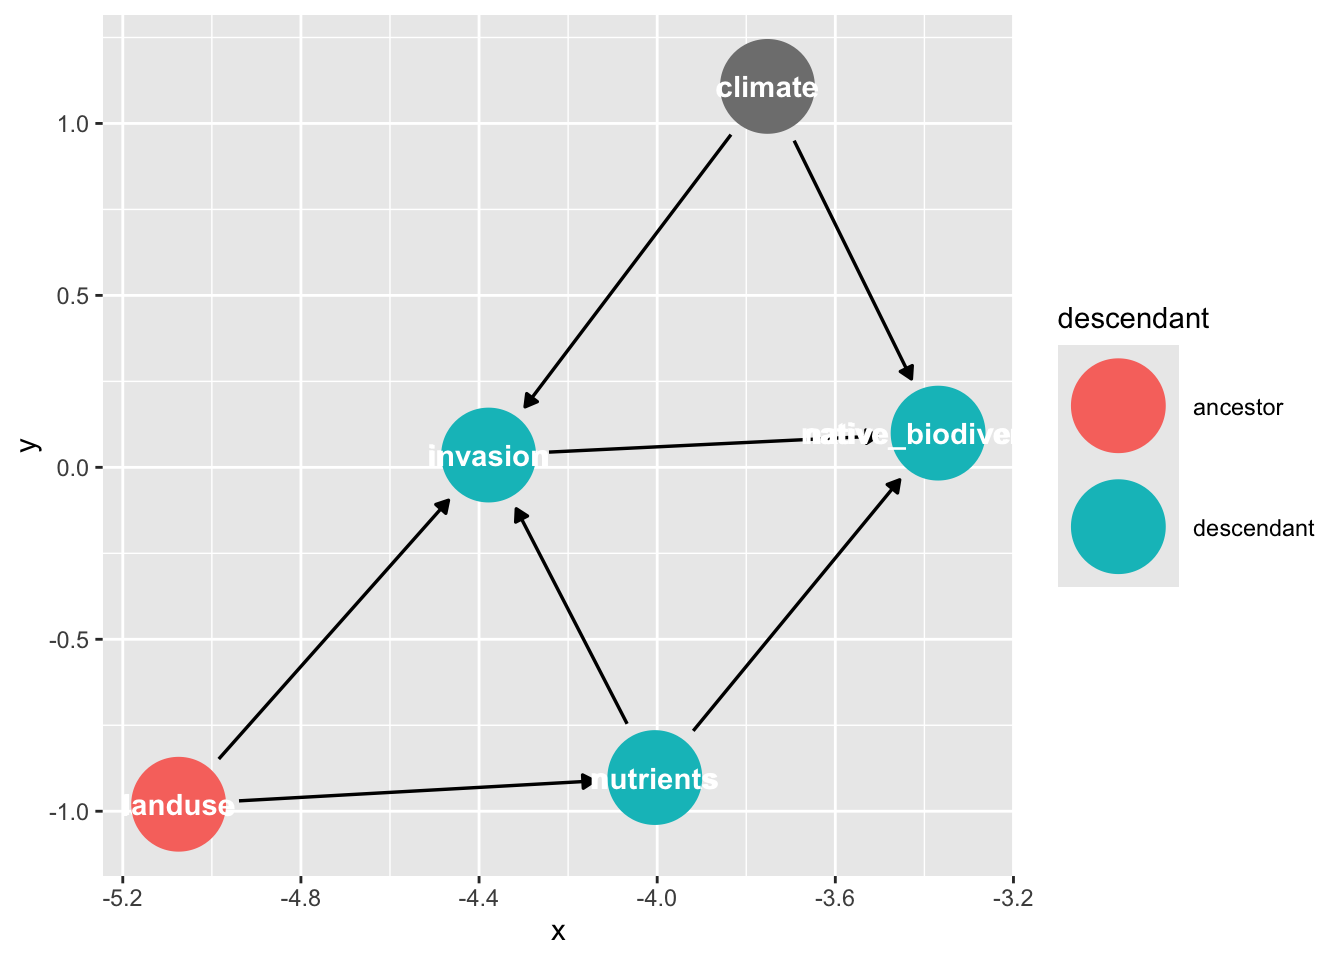
\includegraphics{01_Create_DAG_files/figure-latex/unnamed-chunk-4-1.pdf}

\begin{Shaded}
\begin{Highlighting}[]
\KeywordTok{ggdag_paths}\NormalTok{(DAG_oxygen_under_ice_v2, }\DataTypeTok{shadow =} \OtherTok{TRUE}\NormalTok{) }\CommentTok{#Also, do not forget to set the argument shadow = TRUE, so that the arrows from the adjusted nodes are included}
\end{Highlighting}
\end{Shaded}

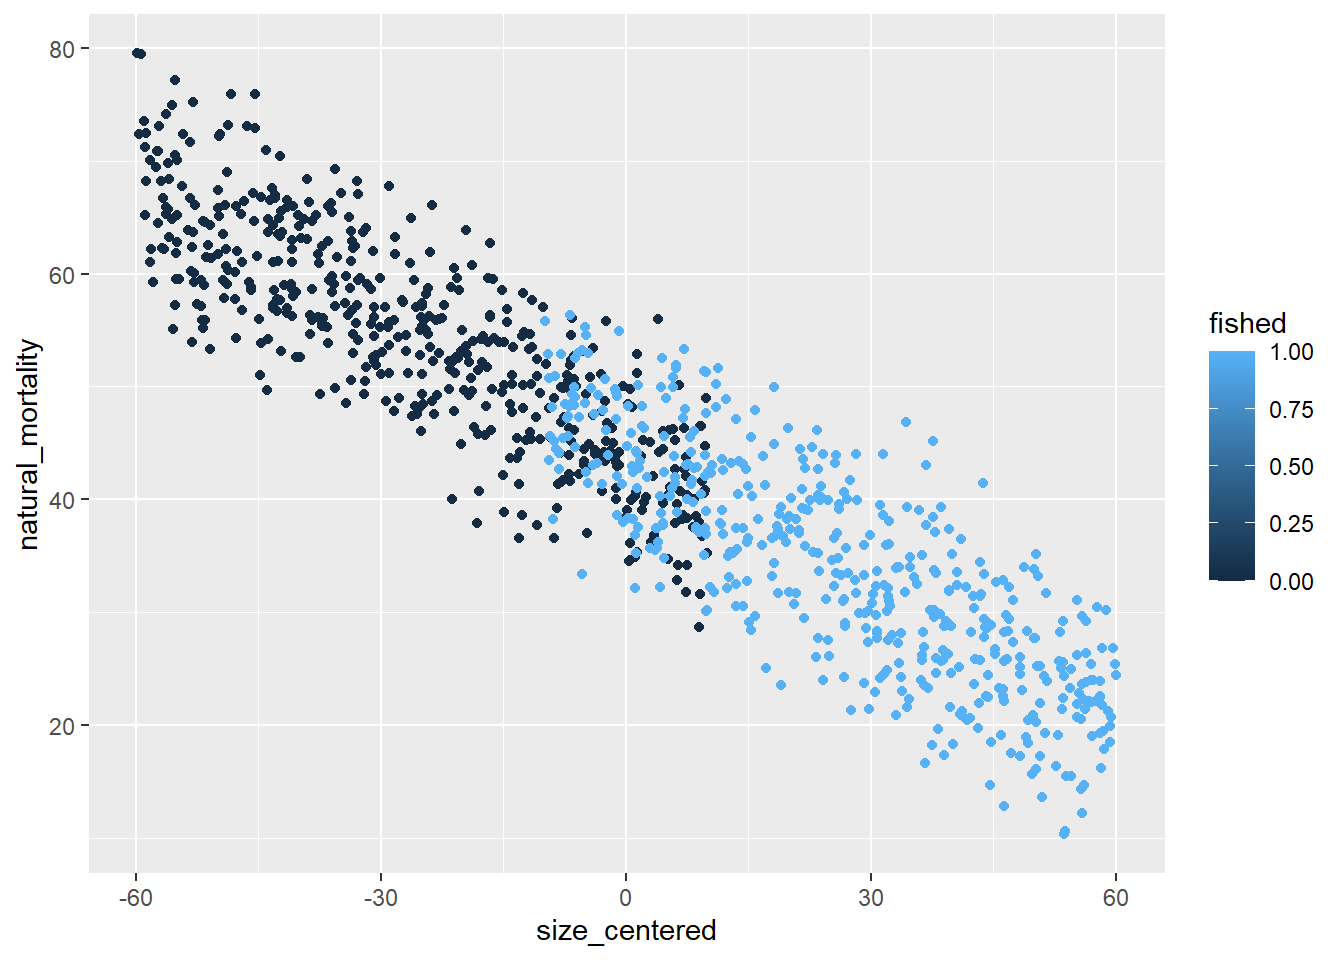
\includegraphics{01_Create_DAG_files/figure-latex/unnamed-chunk-4-2.pdf}

\begin{Shaded}
\begin{Highlighting}[]
\CommentTok{#identify the open paths that need to be adjusted for }
\KeywordTok{paths}\NormalTok{(DAG_oxygen_under_ice_v3)}
\end{Highlighting}
\end{Shaded}

\begin{verbatim}
## $paths
##  [1] "Summer_GPP -> DOC_at_Freeze -> ER_under_ice -> Rate_O2_Drawdown -> anox_duration"                                                                                                                              
##  [2] "Summer_GPP -> DOC_at_Freeze -> ER_under_ice -> Rate_O2_Drawdown <- GPP_under_ice <- Light_Availability <- Ice_Thickness <- Freezing_Degree_Days -> Ice_Duration -> anox_duration"                              
##  [3] "Summer_GPP -> DOC_at_Freeze -> ER_under_ice -> Rate_O2_Drawdown <- GPP_under_ice <- Light_Availability <- Snow_Accumulation -> Ice_Duration -> anox_duration"                                                  
##  [4] "Summer_GPP -> DOC_at_Freeze -> ER_under_ice <- Freezing_Degree_Days -> Ice_Duration -> anox_duration"                                                                                                          
##  [5] "Summer_GPP -> DOC_at_Freeze -> ER_under_ice <- Freezing_Degree_Days -> Ice_Duration <- Snow_Accumulation -> Light_Availability -> GPP_under_ice -> Rate_O2_Drawdown -> anox_duration"                          
##  [6] "Summer_GPP -> DOC_at_Freeze -> ER_under_ice <- Freezing_Degree_Days -> Ice_Thickness -> Light_Availability -> GPP_under_ice -> Rate_O2_Drawdown -> anox_duration"                                              
##  [7] "Summer_GPP -> DOC_at_Freeze -> ER_under_ice <- Freezing_Degree_Days -> Ice_Thickness -> Light_Availability <- Snow_Accumulation -> Ice_Duration -> anox_duration"                                              
##  [8] "Summer_GPP -> GPP_under_ice -> Rate_O2_Drawdown -> anox_duration"                                                                                                                                              
##  [9] "Summer_GPP -> GPP_under_ice -> Rate_O2_Drawdown <- ER_under_ice <- Freezing_Degree_Days -> Ice_Duration -> anox_duration"                                                                                      
## [10] "Summer_GPP -> GPP_under_ice -> Rate_O2_Drawdown <- ER_under_ice <- Freezing_Degree_Days -> Ice_Thickness -> Light_Availability <- Snow_Accumulation -> Ice_Duration -> anox_duration"                          
## [11] "Summer_GPP -> GPP_under_ice <- Light_Availability <- Ice_Thickness <- Freezing_Degree_Days -> ER_under_ice -> Rate_O2_Drawdown -> anox_duration"                                                               
## [12] "Summer_GPP -> GPP_under_ice <- Light_Availability <- Ice_Thickness <- Freezing_Degree_Days -> Ice_Duration -> anox_duration"                                                                                   
## [13] "Summer_GPP -> GPP_under_ice <- Light_Availability <- Snow_Accumulation -> Ice_Duration -> anox_duration"                                                                                                       
## [14] "Summer_GPP -> GPP_under_ice <- Light_Availability <- Snow_Accumulation -> Ice_Duration <- Freezing_Degree_Days -> ER_under_ice -> Rate_O2_Drawdown -> anox_duration"                                           
## [15] "Summer_GPP -> O2_at_Freeze -> anox_duration"                                                                                                                                                                   
## [16] "Summer_GPP <- Terrestrial_DOC_Inputs -> DOC_at_Freeze -> ER_under_ice -> Rate_O2_Drawdown -> anox_duration"                                                                                                    
## [17] "Summer_GPP <- Terrestrial_DOC_Inputs -> DOC_at_Freeze -> ER_under_ice -> Rate_O2_Drawdown <- GPP_under_ice <- Light_Availability <- Ice_Thickness <- Freezing_Degree_Days -> Ice_Duration -> anox_duration"    
## [18] "Summer_GPP <- Terrestrial_DOC_Inputs -> DOC_at_Freeze -> ER_under_ice -> Rate_O2_Drawdown <- GPP_under_ice <- Light_Availability <- Snow_Accumulation -> Ice_Duration -> anox_duration"                        
## [19] "Summer_GPP <- Terrestrial_DOC_Inputs -> DOC_at_Freeze -> ER_under_ice <- Freezing_Degree_Days -> Ice_Duration -> anox_duration"                                                                                
## [20] "Summer_GPP <- Terrestrial_DOC_Inputs -> DOC_at_Freeze -> ER_under_ice <- Freezing_Degree_Days -> Ice_Duration <- Snow_Accumulation -> Light_Availability -> GPP_under_ice -> Rate_O2_Drawdown -> anox_duration"
## [21] "Summer_GPP <- Terrestrial_DOC_Inputs -> DOC_at_Freeze -> ER_under_ice <- Freezing_Degree_Days -> Ice_Thickness -> Light_Availability -> GPP_under_ice -> Rate_O2_Drawdown -> anox_duration"                    
## [22] "Summer_GPP <- Terrestrial_DOC_Inputs -> DOC_at_Freeze -> ER_under_ice <- Freezing_Degree_Days -> Ice_Thickness -> Light_Availability <- Snow_Accumulation -> Ice_Duration -> anox_duration"                    
## 
## $open
##  [1]  TRUE FALSE FALSE FALSE FALSE FALSE FALSE  TRUE FALSE FALSE FALSE FALSE
## [13] FALSE FALSE  TRUE  TRUE FALSE FALSE FALSE FALSE FALSE FALSE
\end{verbatim}

\begin{Shaded}
\begin{Highlighting}[]
\CommentTok{#plot the open  paths }
\KeywordTok{ggdag_paths}\NormalTok{(DAG_oxygen_under_ice_v3)}
\end{Highlighting}
\end{Shaded}

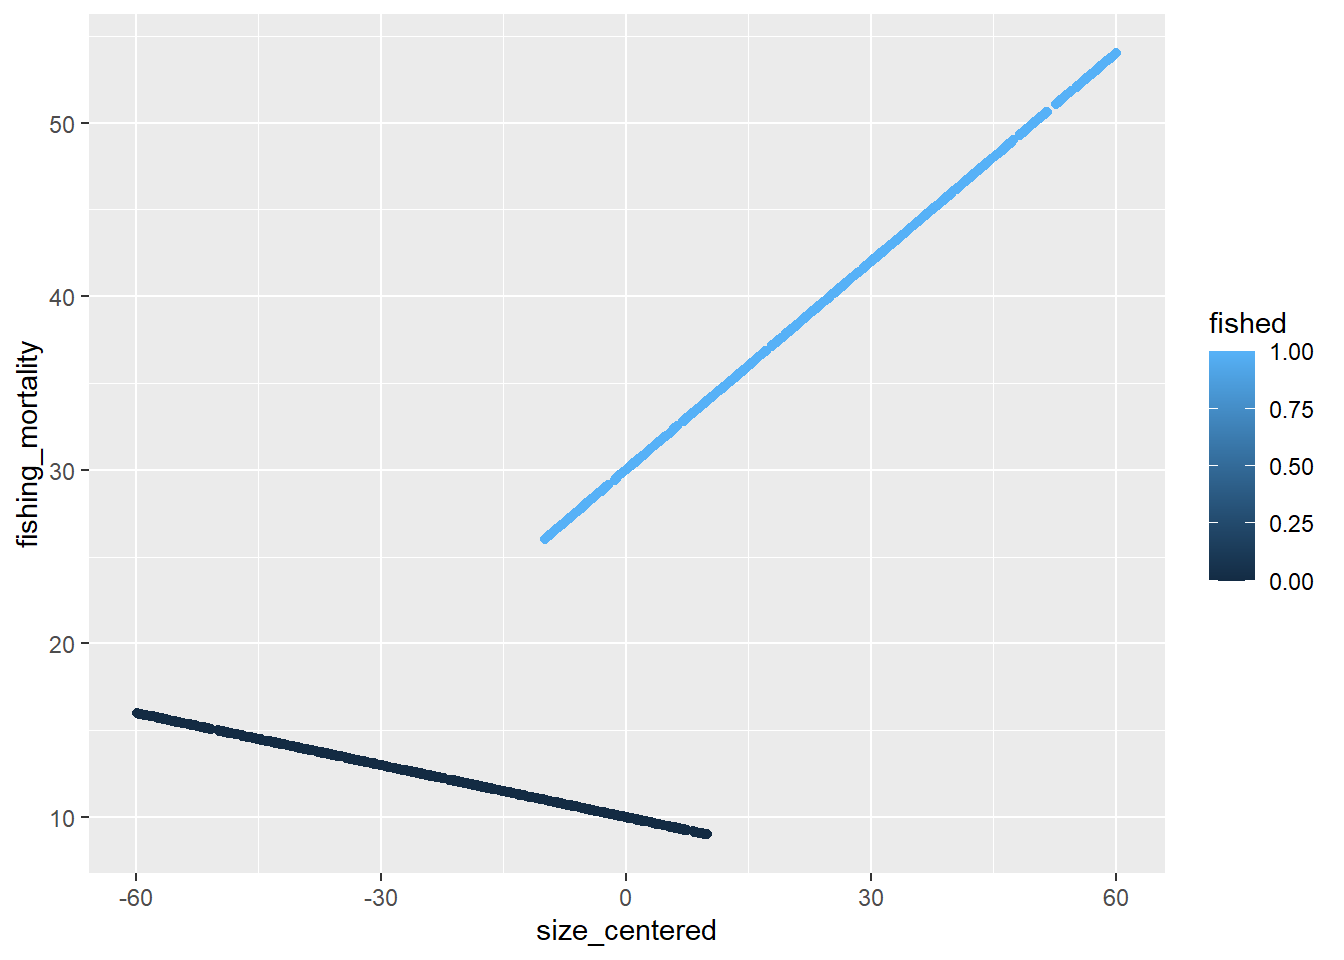
\includegraphics{01_Create_DAG_files/figure-latex/unnamed-chunk-4-3.pdf}

\begin{Shaded}
\begin{Highlighting}[]
\KeywordTok{ggdag_paths}\NormalTok{(DAG_oxygen_under_ice_v3, }\DataTypeTok{shadow =} \OtherTok{TRUE}\NormalTok{) }\CommentTok{#Also, do not forget to set the argument shadow = TRUE, so that the arrows from the adjusted nodes are included}
\end{Highlighting}
\end{Shaded}

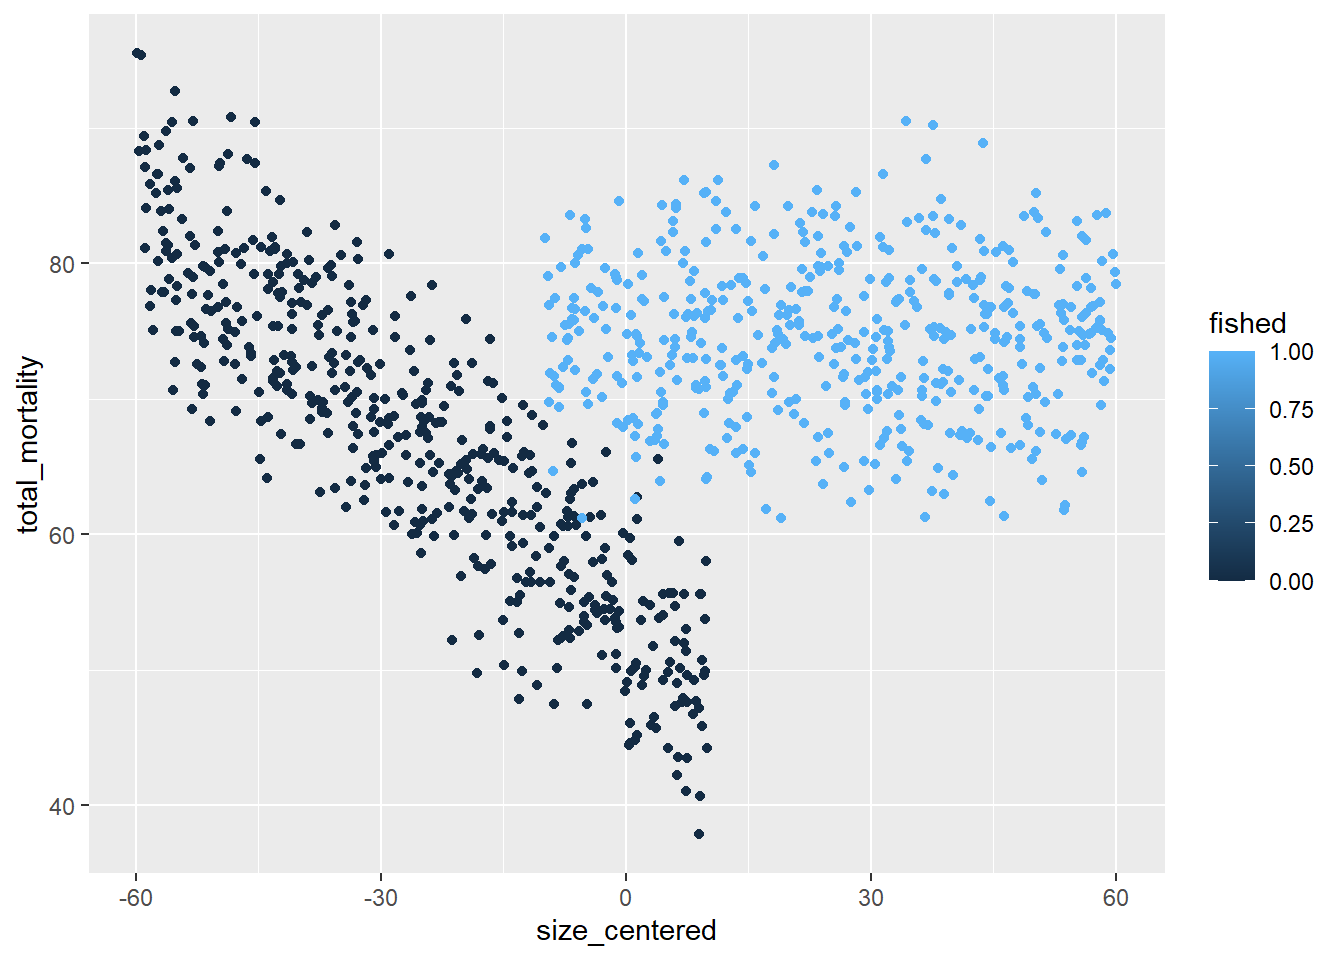
\includegraphics{01_Create_DAG_files/figure-latex/unnamed-chunk-4-4.pdf}
{ {[}\emph{Katie Comment:} Here I have two open paths: Both of these
paths are open and there are mediators along my causal path of interest
from DOC at freeze to anoxic duration. For path {[}1{]} we do not want
to condition on either ER under Ice or Rate of O2 draw down because they
are mediating variables. Looking at paths {[}7{]} and {[}16{]} I have a
slightly confusing structure where summer GPP impacts, DOC at freeze, O2
at freeze, and GPP under ice. In this case I am not sure if I need to
condition on summer GPP? {]} }

{[}1{]} ``DOC\_at\_Freeze -\textgreater{} ER\_under\_ice -\textgreater{}
Rate\_O2\_Drawdown -\textgreater{} anox\_duration'' {[}7{]}
``DOC\_at\_Freeze \textless{}- Summer\_GPP -\textgreater{}
GPP\_under\_ice -\textgreater{} Rate\_O2\_Drawdown -\textgreater{}
anox\_duration'' {[}16{]} ``DOC\_at\_Freeze \textless{}- Summer\_GPP
-\textgreater{} O2\_at\_Freeze -\textgreater{} anox\_duration''

\hypertarget{identify-decendent-nodes}{%
\section{Identify Decendent Nodes}\label{identify-decendent-nodes}}

\begin{Shaded}
\begin{Highlighting}[]
\CommentTok{#you can identify "descendant nodes" }
\KeywordTok{ggdag_descendants}\NormalTok{(DAG_oxygen_under_ice_v2, }\StringTok{"Summer_GPP"}\NormalTok{)}
\end{Highlighting}
\end{Shaded}

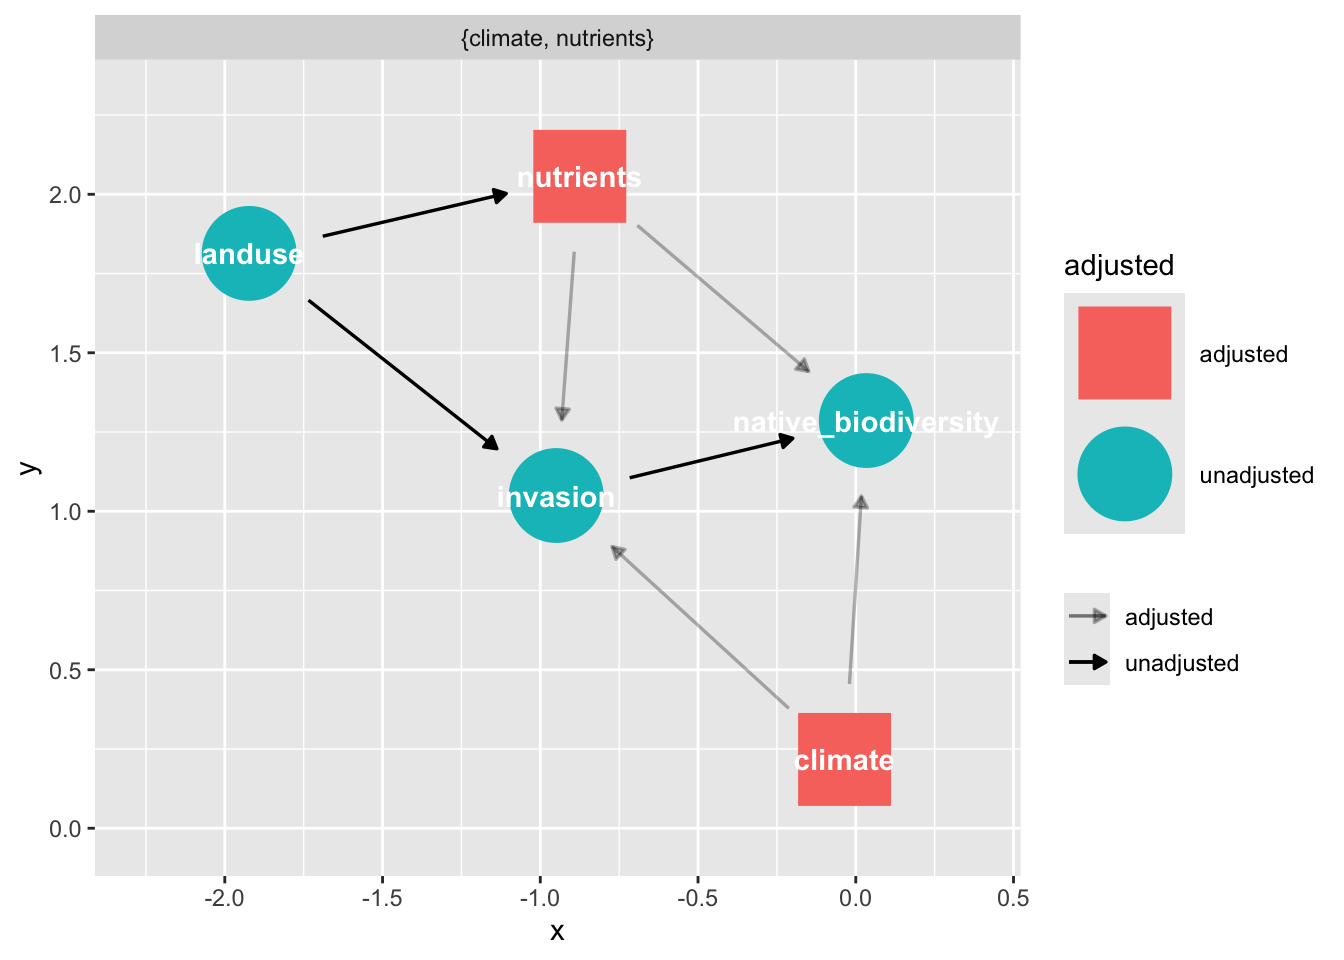
\includegraphics{01_Create_DAG_files/figure-latex/unnamed-chunk-5-1.pdf}

\hypertarget{identify-and-visualize-covariates-that-need-to-be-adjusted-for}{%
\section{Identify and Visualize Covariates that need to be adjusted
for}\label{identify-and-visualize-covariates-that-need-to-be-adjusted-for}}

\begin{Shaded}
\begin{Highlighting}[]
\CommentTok{#identify the covariaters need to be adjusted for to meet the back-door criterion}
\KeywordTok{adjustmentSets}\NormalTok{(DAG_oxygen_under_ice_v2)}
\end{Highlighting}
\end{Shaded}

\begin{verbatim}
## { Freezing_Degree_Days, GPP_under_ice, Ice_Duration, O2_at_Freeze }
## { Freezing_Degree_Days, GPP_under_ice, O2_at_Freeze, Snow_Accumulation
##   }
## { GPP_under_ice, Ice_Thickness, O2_at_Freeze, Snow_Accumulation }
## { GPP_under_ice, Light_Availability, O2_at_Freeze }
## { Summer_GPP }
\end{verbatim}

\begin{Shaded}
\begin{Highlighting}[]
\KeywordTok{adjustmentSets}\NormalTok{(DAG_oxygen_under_ice_v3)}
\end{Highlighting}
\end{Shaded}

\begin{verbatim}
## { Terrestrial_DOC_Inputs }
\end{verbatim}

\begin{Shaded}
\begin{Highlighting}[]
\CommentTok{# Finally, you can also visulaize the variables that need to be adjusted for (which is also told to you by the adjustmentSets() function }
\KeywordTok{ggdag_adjustment_set}\NormalTok{(DAG_oxygen_under_ice_v2, }\DataTypeTok{shadow =} \OtherTok{TRUE}\NormalTok{) }
\end{Highlighting}
\end{Shaded}

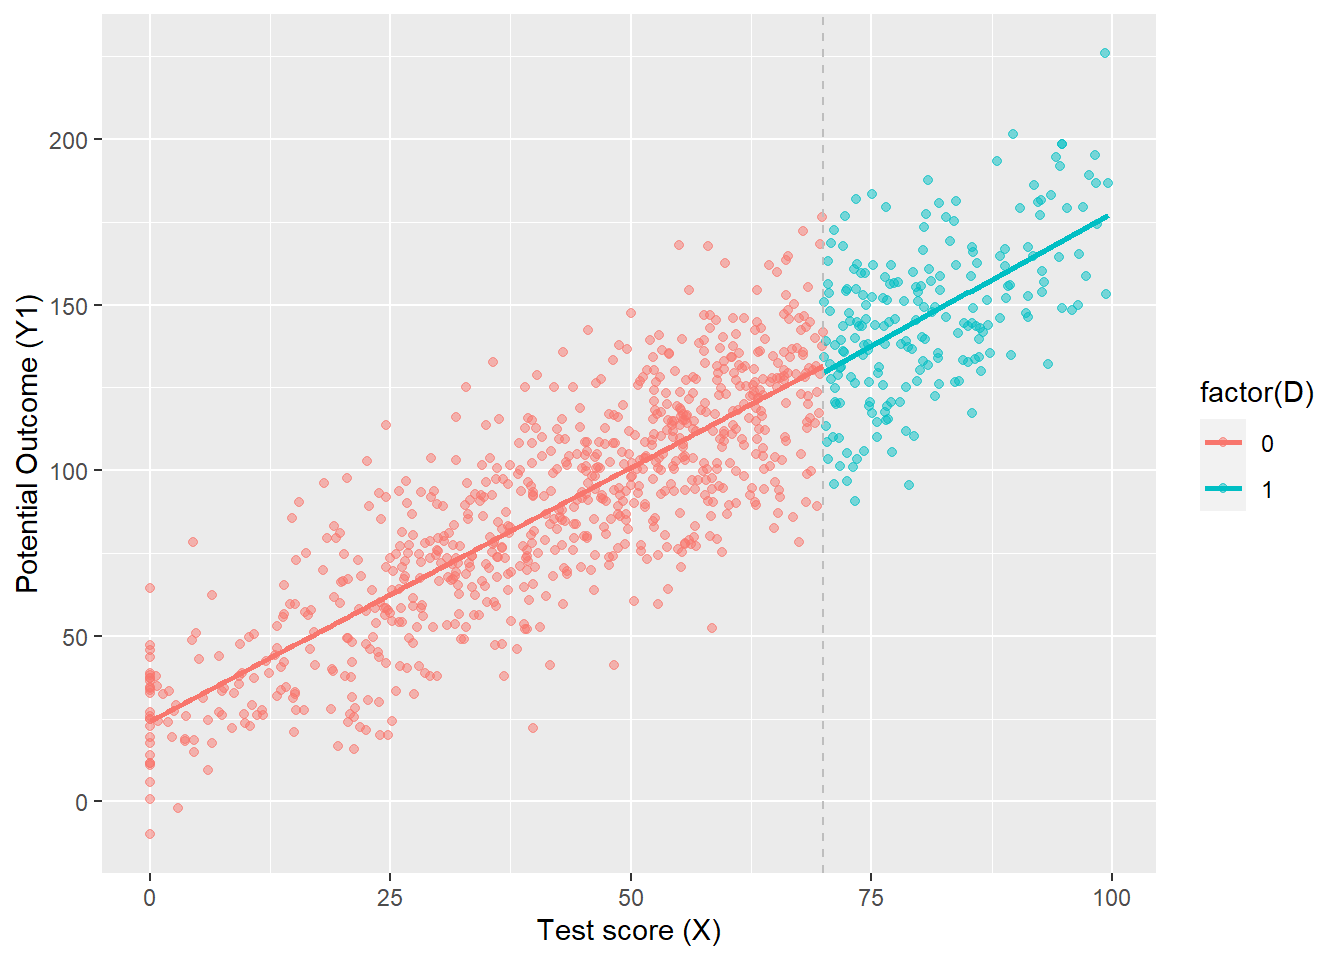
\includegraphics{01_Create_DAG_files/figure-latex/unnamed-chunk-6-1.pdf}

\begin{Shaded}
\begin{Highlighting}[]
\CommentTok{#Also, do not forget to set the argument shadow = TRUE, so that the arrows from the adjusted nodes are included.}
\end{Highlighting}
\end{Shaded}

{ {[}\emph{Katie Comment:} Ahh! I see! This is so handy. It tells me
what I need to condition on. Or at least it gives me options for
pathways that I can condition on to close all of the backdoor. In this
case I would choose to condition on Summer GPP to minimize the number of
variables in my model. That also happens to be super handy because it is
an easy variable to measure (we also have proxies in the form of summer
chlorophyl). Really interesting fiddling with the question I am asking
(``What if the causal question is''how does summer GPP impact anoxic
duration?") and in that case it completely changes the adjustments you
need and there is only one option! In that case we would need to
condition on summer terrestrial DOC inputs {]} }

\#Check Conditional independeces We can also check to see which
variables are conditionally independences in the DAG using
impliedConditionalIndependencies().

\begin{Shaded}
\begin{Highlighting}[]
\CommentTok{# Identify the implied conditional dependencies}
\KeywordTok{impliedConditionalIndependencies}\NormalTok{(DAG_oxygen_under_ice_v2)}
\end{Highlighting}
\end{Shaded}

\begin{verbatim}
## DOC_ _||_ F_D_
## DOC_ _||_ GPP_ | S_GP
## DOC_ _||_ Ic_D
## DOC_ _||_ Ic_T
## DOC_ _||_ Lg_A
## DOC_ _||_ O2__ | S_GP
## DOC_ _||_ R_O2 | ER__, GPP_
## DOC_ _||_ R_O2 | ER__, Lg_A, S_GP
## DOC_ _||_ R_O2 | ER__, Ic_T, S_GP
## DOC_ _||_ R_O2 | ER__, F_D_, S_GP
## DOC_ _||_ Sn_A
## DOC_ _||_ anx_ | Ic_D, O2__, R_O2
## DOC_ _||_ anx_ | F_D_, O2__, R_O2, Sn_A
## DOC_ _||_ anx_ | F_D_, Lg_A, O2__, R_O2
## DOC_ _||_ anx_ | ER__, GPP_, Ic_D, O2__
## DOC_ _||_ anx_ | ER__, F_D_, GPP_, O2__, Sn_A
## DOC_ _||_ anx_ | ER__, F_D_, GPP_, Lg_A, O2__
## DOC_ _||_ anx_ | Ic_D, R_O2, S_GP
## DOC_ _||_ anx_ | ER__, GPP_, Ic_D, S_GP
## DOC_ _||_ anx_ | ER__, Ic_D, Lg_A, S_GP
## DOC_ _||_ anx_ | ER__, Ic_D, Ic_T, Sn_A, S_GP
## DOC_ _||_ anx_ | F_D_, R_O2, Sn_A, S_GP
## DOC_ _||_ anx_ | F_D_, Lg_A, R_O2, S_GP
## DOC_ _||_ anx_ | F_D_, GPP_, R_O2, S_GP
## DOC_ _||_ anx_ | ER__, F_D_, S_GP
## ER__ _||_ GPP_ | Lg_A, S_GP
## ER__ _||_ GPP_ | Ic_T, S_GP
## ER__ _||_ GPP_ | F_D_, S_GP
## ER__ _||_ GPP_ | DOC_, Lg_A
## ER__ _||_ GPP_ | DOC_, Ic_T
## ER__ _||_ GPP_ | DOC_, F_D_
## ER__ _||_ Ic_D | F_D_
## ER__ _||_ Ic_T | F_D_
## ER__ _||_ Lg_A | Ic_T
## ER__ _||_ Lg_A | F_D_
## ER__ _||_ O2__ | S_GP
## ER__ _||_ O2__ | DOC_
## ER__ _||_ Sn_A
## ER__ _||_ S_GP | DOC_
## ER__ _||_ T_DO | DOC_
## ER__ _||_ anx_ | Ic_D, O2__, R_O2
## ER__ _||_ anx_ | F_D_, O2__, R_O2, Sn_A
## ER__ _||_ anx_ | F_D_, Lg_A, O2__, R_O2
## ER__ _||_ anx_ | Ic_D, R_O2, S_GP
## ER__ _||_ anx_ | F_D_, R_O2, Sn_A, S_GP
## ER__ _||_ anx_ | F_D_, Lg_A, R_O2, S_GP
## ER__ _||_ anx_ | F_D_, GPP_, R_O2, S_GP
## ER__ _||_ anx_ | DOC_, GPP_, Ic_D, Lg_A, R_O2
## ER__ _||_ anx_ | DOC_, GPP_, Ic_D, Ic_T, R_O2, Sn_A
## ER__ _||_ anx_ | DOC_, F_D_, GPP_, R_O2
## F_D_ _||_ GPP_ | Lg_A
## F_D_ _||_ GPP_ | Ic_T
## F_D_ _||_ Lg_A | Ic_T
## F_D_ _||_ O2__
## F_D_ _||_ R_O2 | ER__, GPP_
## F_D_ _||_ R_O2 | ER__, Lg_A, S_GP
## F_D_ _||_ R_O2 | DOC_, ER__, Lg_A
## F_D_ _||_ R_O2 | ER__, Ic_T, S_GP
## F_D_ _||_ R_O2 | DOC_, ER__, Ic_T
## F_D_ _||_ Sn_A
## F_D_ _||_ S_GP
## F_D_ _||_ T_DO
## F_D_ _||_ anx_ | Ic_D, O2__, R_O2
## F_D_ _||_ anx_ | ER__, GPP_, Ic_D, O2__
## F_D_ _||_ anx_ | Ic_D, R_O2, S_GP
## F_D_ _||_ anx_ | ER__, GPP_, Ic_D, S_GP
## F_D_ _||_ anx_ | DOC_, GPP_, Ic_D, Lg_A, R_O2
## F_D_ _||_ anx_ | ER__, Ic_D, Lg_A, S_GP
## F_D_ _||_ anx_ | DOC_, ER__, Ic_D, Lg_A
## F_D_ _||_ anx_ | DOC_, GPP_, Ic_D, Ic_T, R_O2, Sn_A
## F_D_ _||_ anx_ | ER__, Ic_D, Ic_T, Sn_A, S_GP
## F_D_ _||_ anx_ | DOC_, ER__, Ic_D, Ic_T, Sn_A
## GPP_ _||_ Ic_D | F_D_, Sn_A
## GPP_ _||_ Ic_D | Ic_T, Sn_A
## GPP_ _||_ Ic_D | Lg_A
## GPP_ _||_ Ic_T | Lg_A
## GPP_ _||_ O2__ | S_GP
## GPP_ _||_ Sn_A | Lg_A
## GPP_ _||_ T_DO | S_GP
## GPP_ _||_ anx_ | Ic_D, O2__, R_O2
## GPP_ _||_ anx_ | F_D_, O2__, R_O2, Sn_A
## GPP_ _||_ anx_ | F_D_, Lg_A, O2__, R_O2
## GPP_ _||_ anx_ | Ic_D, R_O2, S_GP
## GPP_ _||_ anx_ | F_D_, R_O2, Sn_A, S_GP
## GPP_ _||_ anx_ | F_D_, Lg_A, R_O2, S_GP
## GPP_ _||_ anx_ | DOC_, ER__, Ic_T, O2__, R_O2, Sn_A
## GPP_ _||_ anx_ | ER__, Ic_T, R_O2, Sn_A, S_GP
## GPP_ _||_ anx_ | DOC_, ER__, Lg_A, O2__, R_O2
## GPP_ _||_ anx_ | ER__, Lg_A, R_O2, S_GP
## Ic_D _||_ Ic_T | F_D_
## Ic_D _||_ Lg_A | Ic_T, Sn_A
## Ic_D _||_ Lg_A | F_D_, Sn_A
## Ic_D _||_ O2__
## Ic_D _||_ R_O2 | ER__, GPP_
## Ic_D _||_ R_O2 | ER__, Lg_A, S_GP
## Ic_D _||_ R_O2 | DOC_, ER__, Lg_A
## Ic_D _||_ R_O2 | ER__, Ic_T, Sn_A, S_GP
## Ic_D _||_ R_O2 | DOC_, ER__, Ic_T, Sn_A
## Ic_D _||_ R_O2 | DOC_, F_D_, GPP_
## Ic_D _||_ R_O2 | F_D_, GPP_, S_GP
## Ic_D _||_ R_O2 | F_D_, Lg_A
## Ic_D _||_ R_O2 | F_D_, Sn_A
## Ic_D _||_ S_GP
## Ic_D _||_ T_DO
## Ic_T _||_ O2__
## Ic_T _||_ R_O2 | ER__, GPP_
## Ic_T _||_ R_O2 | DOC_, F_D_, GPP_
## Ic_T _||_ R_O2 | F_D_, GPP_, S_GP
## Ic_T _||_ R_O2 | ER__, Lg_A, S_GP
## Ic_T _||_ R_O2 | DOC_, ER__, Lg_A
## Ic_T _||_ R_O2 | F_D_, Lg_A
## Ic_T _||_ Sn_A
## Ic_T _||_ S_GP
## Ic_T _||_ T_DO
## Ic_T _||_ anx_ | Ic_D, O2__, R_O2
## Ic_T _||_ anx_ | ER__, GPP_, Ic_D, O2__
## Ic_T _||_ anx_ | DOC_, F_D_, GPP_, Ic_D, O2__
## Ic_T _||_ anx_ | Ic_D, R_O2, S_GP
## Ic_T _||_ anx_ | ER__, GPP_, Ic_D, S_GP
## Ic_T _||_ anx_ | F_D_, GPP_, Ic_D, S_GP
## Ic_T _||_ anx_ | DOC_, GPP_, Ic_D, Lg_A, R_O2
## Ic_T _||_ anx_ | ER__, Ic_D, Lg_A, S_GP
## Ic_T _||_ anx_ | DOC_, ER__, Ic_D, Lg_A
## Ic_T _||_ anx_ | F_D_, Ic_D, Lg_A
## Ic_T _||_ anx_ | F_D_, O2__, R_O2, Sn_A
## Ic_T _||_ anx_ | ER__, F_D_, GPP_, O2__, Sn_A
## Ic_T _||_ anx_ | DOC_, F_D_, GPP_, O2__, Sn_A
## Ic_T _||_ anx_ | F_D_, R_O2, Sn_A, S_GP
## Ic_T _||_ anx_ | F_D_, GPP_, Sn_A, S_GP
## Ic_T _||_ anx_ | F_D_, Lg_A, Sn_A
## Lg_A _||_ O2__
## Lg_A _||_ R_O2 | ER__, GPP_
## Lg_A _||_ R_O2 | DOC_, F_D_, GPP_
## Lg_A _||_ R_O2 | F_D_, GPP_, S_GP
## Lg_A _||_ R_O2 | DOC_, GPP_, Ic_T
## Lg_A _||_ R_O2 | GPP_, Ic_T, S_GP
## Lg_A _||_ S_GP
## Lg_A _||_ T_DO
## Lg_A _||_ anx_ | Ic_D, O2__, R_O2
## Lg_A _||_ anx_ | ER__, GPP_, Ic_D, O2__
## Lg_A _||_ anx_ | F_D_, O2__, R_O2, Sn_A
## Lg_A _||_ anx_ | ER__, F_D_, GPP_, O2__, Sn_A
## Lg_A _||_ anx_ | DOC_, ER__, Ic_T, O2__, R_O2, Sn_A
## Lg_A _||_ anx_ | DOC_, F_D_, GPP_, Ic_D, O2__
## Lg_A _||_ anx_ | DOC_, F_D_, GPP_, O2__, Sn_A
## Lg_A _||_ anx_ | DOC_, GPP_, Ic_T, O2__, Sn_A
## Lg_A _||_ anx_ | Ic_D, R_O2, S_GP
## Lg_A _||_ anx_ | F_D_, R_O2, Sn_A, S_GP
## Lg_A _||_ anx_ | ER__, Ic_T, R_O2, Sn_A, S_GP
## Lg_A _||_ anx_ | ER__, GPP_, Ic_D, S_GP
## Lg_A _||_ anx_ | F_D_, GPP_, Ic_D, S_GP
## Lg_A _||_ anx_ | F_D_, GPP_, Sn_A, S_GP
## Lg_A _||_ anx_ | GPP_, Ic_T, Sn_A, S_GP
## O2__ _||_ R_O2 | ER__, GPP_
## O2__ _||_ R_O2 | DOC_, F_D_, GPP_
## O2__ _||_ R_O2 | DOC_, GPP_, Ic_T
## O2__ _||_ R_O2 | DOC_, GPP_, Lg_A
## O2__ _||_ R_O2 | S_GP
## O2__ _||_ Sn_A
## O2__ _||_ T_DO | S_GP
## R_O2 _||_ Sn_A | Ic_T, Lg_A
## R_O2 _||_ Sn_A | F_D_, Lg_A
## R_O2 _||_ Sn_A | GPP_, Ic_T, S_GP
## R_O2 _||_ Sn_A | F_D_, GPP_, S_GP
## R_O2 _||_ Sn_A | DOC_, GPP_, Ic_T
## R_O2 _||_ Sn_A | DOC_, F_D_, GPP_
## R_O2 _||_ Sn_A | DOC_, ER__, Lg_A
## R_O2 _||_ Sn_A | ER__, Lg_A, S_GP
## R_O2 _||_ Sn_A | ER__, GPP_
## R_O2 _||_ S_GP | DOC_, GPP_, Lg_A
## R_O2 _||_ S_GP | DOC_, GPP_, Ic_T
## R_O2 _||_ S_GP | DOC_, F_D_, GPP_
## R_O2 _||_ S_GP | ER__, GPP_
## R_O2 _||_ T_DO | DOC_, S_GP
## R_O2 _||_ T_DO | DOC_, GPP_, Lg_A
## R_O2 _||_ T_DO | DOC_, GPP_, Ic_T
## R_O2 _||_ T_DO | DOC_, F_D_, GPP_
## R_O2 _||_ T_DO | ER__, F_D_, S_GP
## R_O2 _||_ T_DO | ER__, Ic_T, S_GP
## R_O2 _||_ T_DO | ER__, Lg_A, S_GP
## R_O2 _||_ T_DO | ER__, GPP_
## Sn_A _||_ S_GP
## Sn_A _||_ T_DO
## Sn_A _||_ anx_ | Ic_D, O2__, R_O2
## Sn_A _||_ anx_ | ER__, GPP_, Ic_D, O2__
## Sn_A _||_ anx_ | Ic_D, R_O2, S_GP
## Sn_A _||_ anx_ | ER__, GPP_, Ic_D, S_GP
## Sn_A _||_ anx_ | DOC_, F_D_, GPP_, Ic_D, O2__
## Sn_A _||_ anx_ | F_D_, GPP_, Ic_D, S_GP
## Sn_A _||_ anx_ | DOC_, GPP_, Ic_D, Lg_A, R_O2
## Sn_A _||_ anx_ | ER__, Ic_D, Lg_A, S_GP
## Sn_A _||_ anx_ | DOC_, ER__, Ic_D, Lg_A
## Sn_A _||_ anx_ | F_D_, Ic_D, Lg_A
## S_GP _||_ anx_ | Ic_D, O2__, R_O2
## S_GP _||_ anx_ | ER__, GPP_, Ic_D, O2__
## S_GP _||_ anx_ | F_D_, O2__, R_O2, Sn_A
## S_GP _||_ anx_ | F_D_, Lg_A, O2__, R_O2
## S_GP _||_ anx_ | ER__, F_D_, GPP_, O2__, Sn_A
## S_GP _||_ anx_ | ER__, F_D_, GPP_, Lg_A, O2__
## S_GP _||_ anx_ | DOC_, ER__, Ic_T, O2__, R_O2, Sn_A
## S_GP _||_ anx_ | DOC_, ER__, Lg_A, O2__, R_O2
## S_GP _||_ anx_ | DOC_, F_D_, GPP_, Ic_D, O2__
## S_GP _||_ anx_ | DOC_, F_D_, GPP_, O2__, Sn_A
## S_GP _||_ anx_ | DOC_, GPP_, Ic_T, O2__, Sn_A
## S_GP _||_ anx_ | DOC_, GPP_, Lg_A, O2__
## T_DO _||_ anx_ | Ic_D, O2__, R_O2
## T_DO _||_ anx_ | F_D_, O2__, R_O2, Sn_A
## T_DO _||_ anx_ | F_D_, Lg_A, O2__, R_O2
## T_DO _||_ anx_ | DOC_, ER__, Ic_T, O2__, R_O2, Sn_A
## T_DO _||_ anx_ | DOC_, ER__, Lg_A, O2__, R_O2
## T_DO _||_ anx_ | ER__, GPP_, Ic_D, O2__
## T_DO _||_ anx_ | ER__, F_D_, GPP_, O2__, Sn_A
## T_DO _||_ anx_ | ER__, F_D_, GPP_, Lg_A, O2__
## T_DO _||_ anx_ | DOC_, F_D_, GPP_, Ic_D, O2__
## T_DO _||_ anx_ | DOC_, F_D_, GPP_, O2__, Sn_A
## T_DO _||_ anx_ | DOC_, GPP_, Ic_T, O2__, Sn_A
## T_DO _||_ anx_ | DOC_, GPP_, Lg_A, O2__
## T_DO _||_ anx_ | Ic_D, R_O2, S_GP
## T_DO _||_ anx_ | ER__, GPP_, Ic_D, S_GP
## T_DO _||_ anx_ | ER__, Ic_D, Lg_A, S_GP
## T_DO _||_ anx_ | ER__, Ic_D, Ic_T, Sn_A, S_GP
## T_DO _||_ anx_ | F_D_, R_O2, Sn_A, S_GP
## T_DO _||_ anx_ | F_D_, Lg_A, R_O2, S_GP
## T_DO _||_ anx_ | F_D_, GPP_, R_O2, S_GP
## T_DO _||_ anx_ | ER__, F_D_, S_GP
## T_DO _||_ anx_ | DOC_, S_GP
\end{verbatim}

{ {[}\emph{Katie Comment:} Well that is a terrifyingly long list of
conditional indipendicies. I think that I might need to more explicitly
time step some of my variables. For example GPP and ER do impact
eachother in each direction. So I need to specify GPP of the previous
summer impacting ER under ice in winter etc.{]} }

{ {[}\emph{Questions:} Including lake and year as random effects?{]}}

\end{document}
